% Created by tikzDevice version 0.12.6 on 2025-02-15 09:46:31
% !TEX encoding = UTF-8 Unicode
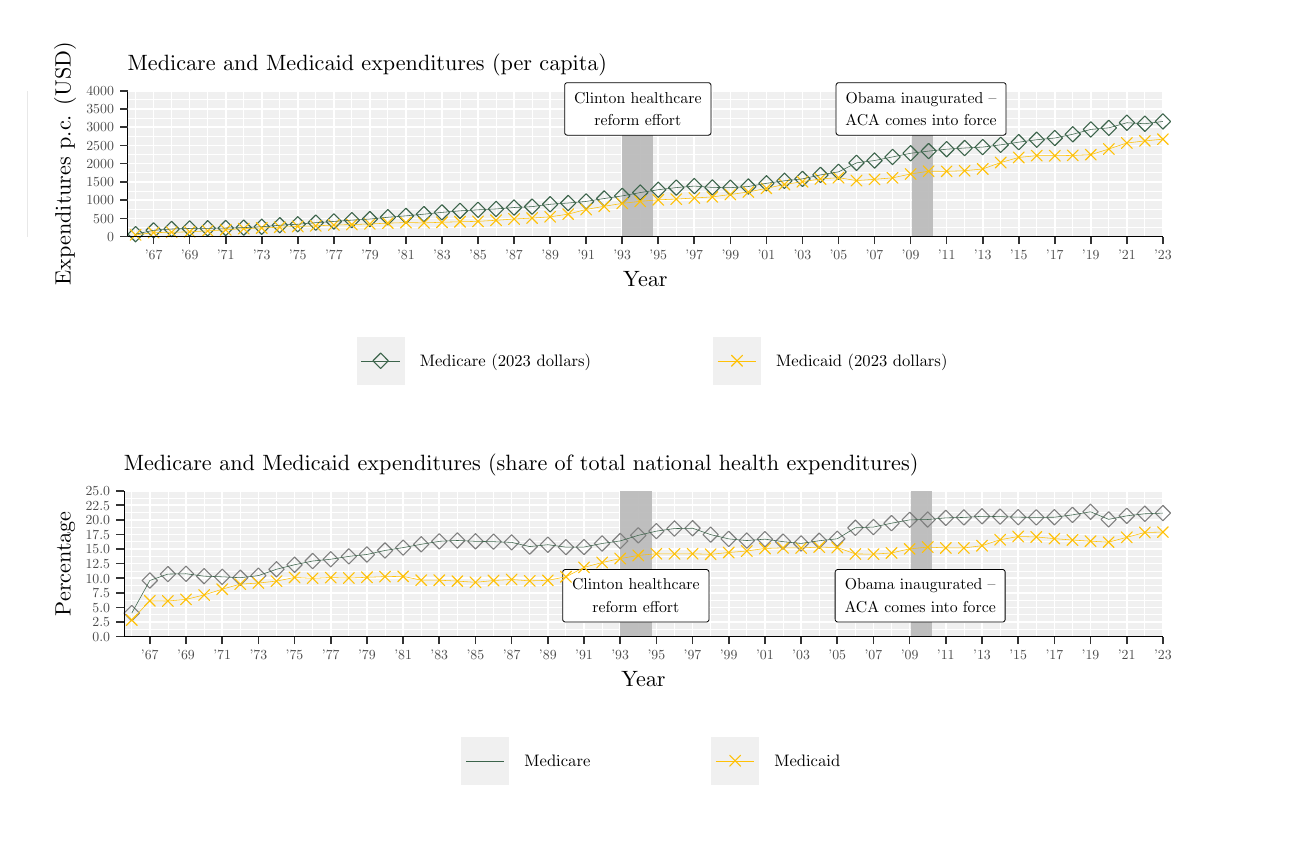
\begin{tikzpicture}[x=1pt,y=1pt]
\definecolor{fillColor}{RGB}{255,255,255}
\path[use as bounding box,fill=fillColor,fill opacity=0.00] (0,0) rectangle (455.30,289.08);
\begin{scope}
\path[clip] (  0.00,144.54) rectangle (455.30,289.08);
\definecolor{drawColor}{RGB}{255,255,255}
\definecolor{fillColor}{RGB}{255,255,255}

\path[draw=drawColor,line width= 0.6pt,line join=round,line cap=round,fill=fillColor] (  0.00,144.54) rectangle (455.30,289.08);
\end{scope}
\begin{scope}
\path[clip] (  0.00,  0.00) rectangle (455.30,289.08);
\definecolor{fillColor}{gray}{0.94}

\path[fill=fillColor] ( 36.14,213.57) rectangle (410.30,266.30);
\definecolor{drawColor}{RGB}{255,255,255}

\path[draw=drawColor,line width= 0.3pt,line join=round] ( 36.14,216.86) --
	(410.30,216.86);

\path[draw=drawColor,line width= 0.3pt,line join=round] ( 36.14,223.46) --
	(410.30,223.46);

\path[draw=drawColor,line width= 0.3pt,line join=round] ( 36.14,230.05) --
	(410.30,230.05);

\path[draw=drawColor,line width= 0.3pt,line join=round] ( 36.14,236.64) --
	(410.30,236.64);

\path[draw=drawColor,line width= 0.3pt,line join=round] ( 36.14,243.23) --
	(410.30,243.23);

\path[draw=drawColor,line width= 0.3pt,line join=round] ( 36.14,249.82) --
	(410.30,249.82);

\path[draw=drawColor,line width= 0.3pt,line join=round] ( 36.14,256.42) --
	(410.30,256.42);

\path[draw=drawColor,line width= 0.3pt,line join=round] ( 36.14,263.01) --
	(410.30,263.01);

\path[draw=drawColor,line width= 0.3pt,line join=round] ( 38.99,213.57) --
	( 38.99,266.30);

\path[draw=drawColor,line width= 0.3pt,line join=round] ( 52.02,213.57) --
	( 52.02,266.30);

\path[draw=drawColor,line width= 0.3pt,line join=round] ( 65.04,213.57) --
	( 65.04,266.30);

\path[draw=drawColor,line width= 0.3pt,line join=round] ( 78.07,213.57) --
	( 78.07,266.30);

\path[draw=drawColor,line width= 0.3pt,line join=round] ( 91.09,213.57) --
	( 91.09,266.30);

\path[draw=drawColor,line width= 0.3pt,line join=round] (104.12,213.57) --
	(104.12,266.30);

\path[draw=drawColor,line width= 0.3pt,line join=round] (117.14,213.57) --
	(117.14,266.30);

\path[draw=drawColor,line width= 0.3pt,line join=round] (130.17,213.57) --
	(130.17,266.30);

\path[draw=drawColor,line width= 0.3pt,line join=round] (143.19,213.57) --
	(143.19,266.30);

\path[draw=drawColor,line width= 0.3pt,line join=round] (156.22,213.57) --
	(156.22,266.30);

\path[draw=drawColor,line width= 0.3pt,line join=round] (169.25,213.57) --
	(169.25,266.30);

\path[draw=drawColor,line width= 0.3pt,line join=round] (182.27,213.57) --
	(182.27,266.30);

\path[draw=drawColor,line width= 0.3pt,line join=round] (195.30,213.57) --
	(195.30,266.30);

\path[draw=drawColor,line width= 0.3pt,line join=round] (208.32,213.57) --
	(208.32,266.30);

\path[draw=drawColor,line width= 0.3pt,line join=round] (221.35,213.57) --
	(221.35,266.30);

\path[draw=drawColor,line width= 0.3pt,line join=round] (234.37,213.57) --
	(234.37,266.30);

\path[draw=drawColor,line width= 0.3pt,line join=round] (247.40,213.57) --
	(247.40,266.30);

\path[draw=drawColor,line width= 0.3pt,line join=round] (260.42,213.57) --
	(260.42,266.30);

\path[draw=drawColor,line width= 0.3pt,line join=round] (273.45,213.57) --
	(273.45,266.30);

\path[draw=drawColor,line width= 0.3pt,line join=round] (286.47,213.57) --
	(286.47,266.30);

\path[draw=drawColor,line width= 0.3pt,line join=round] (299.50,213.57) --
	(299.50,266.30);

\path[draw=drawColor,line width= 0.3pt,line join=round] (312.53,213.57) --
	(312.53,266.30);

\path[draw=drawColor,line width= 0.3pt,line join=round] (325.55,213.57) --
	(325.55,266.30);

\path[draw=drawColor,line width= 0.3pt,line join=round] (338.58,213.57) --
	(338.58,266.30);

\path[draw=drawColor,line width= 0.3pt,line join=round] (351.60,213.57) --
	(351.60,266.30);

\path[draw=drawColor,line width= 0.3pt,line join=round] (364.63,213.57) --
	(364.63,266.30);

\path[draw=drawColor,line width= 0.3pt,line join=round] (377.65,213.57) --
	(377.65,266.30);

\path[draw=drawColor,line width= 0.3pt,line join=round] (390.68,213.57) --
	(390.68,266.30);

\path[draw=drawColor,line width= 0.3pt,line join=round] (403.70,213.57) --
	(403.70,266.30);

\path[draw=drawColor,line width= 0.6pt,line join=round] ( 36.14,213.57) --
	(410.30,213.57);

\path[draw=drawColor,line width= 0.6pt,line join=round] ( 36.14,220.16) --
	(410.30,220.16);

\path[draw=drawColor,line width= 0.6pt,line join=round] ( 36.14,226.75) --
	(410.30,226.75);

\path[draw=drawColor,line width= 0.6pt,line join=round] ( 36.14,233.34) --
	(410.30,233.34);

\path[draw=drawColor,line width= 0.6pt,line join=round] ( 36.14,239.94) --
	(410.30,239.94);

\path[draw=drawColor,line width= 0.6pt,line join=round] ( 36.14,246.53) --
	(410.30,246.53);

\path[draw=drawColor,line width= 0.6pt,line join=round] ( 36.14,253.12) --
	(410.30,253.12);

\path[draw=drawColor,line width= 0.6pt,line join=round] ( 36.14,259.71) --
	(410.30,259.71);

\path[draw=drawColor,line width= 0.6pt,line join=round] ( 36.14,266.30) --
	(410.30,266.30);

\path[draw=drawColor,line width= 0.6pt,line join=round] ( 45.50,213.57) --
	( 45.50,266.30);

\path[draw=drawColor,line width= 0.6pt,line join=round] ( 58.53,213.57) --
	( 58.53,266.30);

\path[draw=drawColor,line width= 0.6pt,line join=round] ( 71.55,213.57) --
	( 71.55,266.30);

\path[draw=drawColor,line width= 0.6pt,line join=round] ( 84.58,213.57) --
	( 84.58,266.30);

\path[draw=drawColor,line width= 0.6pt,line join=round] ( 97.60,213.57) --
	( 97.60,266.30);

\path[draw=drawColor,line width= 0.6pt,line join=round] (110.64,213.57) --
	(110.64,266.30);

\path[draw=drawColor,line width= 0.6pt,line join=round] (123.65,213.57) --
	(123.65,266.30);

\path[draw=drawColor,line width= 0.6pt,line join=round] (136.69,213.57) --
	(136.69,266.30);

\path[draw=drawColor,line width= 0.6pt,line join=round] (149.70,213.57) --
	(149.70,266.30);

\path[draw=drawColor,line width= 0.6pt,line join=round] (162.74,213.57) --
	(162.74,266.30);

\path[draw=drawColor,line width= 0.6pt,line join=round] (175.75,213.57) --
	(175.75,266.30);

\path[draw=drawColor,line width= 0.6pt,line join=round] (188.79,213.57) --
	(188.79,266.30);

\path[draw=drawColor,line width= 0.6pt,line join=round] (201.80,213.57) --
	(201.80,266.30);

\path[draw=drawColor,line width= 0.6pt,line join=round] (214.84,213.57) --
	(214.84,266.30);

\path[draw=drawColor,line width= 0.6pt,line join=round] (227.86,213.57) --
	(227.86,266.30);

\path[draw=drawColor,line width= 0.6pt,line join=round] (240.89,213.57) --
	(240.89,266.30);

\path[draw=drawColor,line width= 0.6pt,line join=round] (253.91,213.57) --
	(253.91,266.30);

\path[draw=drawColor,line width= 0.6pt,line join=round] (266.94,213.57) --
	(266.94,266.30);

\path[draw=drawColor,line width= 0.6pt,line join=round] (279.96,213.57) --
	(279.96,266.30);

\path[draw=drawColor,line width= 0.6pt,line join=round] (292.99,213.57) --
	(292.99,266.30);

\path[draw=drawColor,line width= 0.6pt,line join=round] (306.01,213.57) --
	(306.01,266.30);

\path[draw=drawColor,line width= 0.6pt,line join=round] (319.04,213.57) --
	(319.04,266.30);

\path[draw=drawColor,line width= 0.6pt,line join=round] (332.06,213.57) --
	(332.06,266.30);

\path[draw=drawColor,line width= 0.6pt,line join=round] (345.09,213.57) --
	(345.09,266.30);

\path[draw=drawColor,line width= 0.6pt,line join=round] (358.11,213.57) --
	(358.11,266.30);

\path[draw=drawColor,line width= 0.6pt,line join=round] (371.14,213.57) --
	(371.14,266.30);

\path[draw=drawColor,line width= 0.6pt,line join=round] (384.16,213.57) --
	(384.16,266.30);

\path[draw=drawColor,line width= 0.6pt,line join=round] (397.20,213.57) --
	(397.20,266.30);

\path[draw=drawColor,line width= 0.6pt,line join=round] (410.21,213.57) --
	(410.21,266.30);
\definecolor{drawColor}{RGB}{190,190,190}

\path[draw=drawColor,line width= 0.6pt,line join=round] ( -0.09,213.57) -- ( -0.09,266.30);
\definecolor{fillColor}{RGB}{190,190,190}

\path[fill=fillColor,fill opacity=0.01] (214.84,213.57) rectangle (226.13,266.30);

\path[fill=fillColor,fill opacity=0.01] (214.84,213.57) rectangle (226.13,266.30);

\path[fill=fillColor,fill opacity=0.01] (214.84,213.57) rectangle (226.13,266.30);

\path[fill=fillColor,fill opacity=0.01] (214.84,213.57) rectangle (226.13,266.30);

\path[fill=fillColor,fill opacity=0.01] (214.84,213.57) rectangle (226.13,266.30);

\path[fill=fillColor,fill opacity=0.01] (214.84,213.57) rectangle (226.13,266.30);

\path[fill=fillColor,fill opacity=0.01] (214.84,213.57) rectangle (226.13,266.30);

\path[fill=fillColor,fill opacity=0.01] (214.84,213.57) rectangle (226.13,266.30);

\path[fill=fillColor,fill opacity=0.01] (214.84,213.57) rectangle (226.13,266.30);

\path[fill=fillColor,fill opacity=0.01] (214.84,213.57) rectangle (226.13,266.30);

\path[fill=fillColor,fill opacity=0.01] (214.84,213.57) rectangle (226.13,266.30);

\path[fill=fillColor,fill opacity=0.01] (214.84,213.57) rectangle (226.13,266.30);

\path[fill=fillColor,fill opacity=0.01] (214.84,213.57) rectangle (226.13,266.30);

\path[fill=fillColor,fill opacity=0.01] (214.84,213.57) rectangle (226.13,266.30);

\path[fill=fillColor,fill opacity=0.01] (214.84,213.57) rectangle (226.13,266.30);

\path[fill=fillColor,fill opacity=0.01] (214.84,213.57) rectangle (226.13,266.30);

\path[fill=fillColor,fill opacity=0.01] (214.84,213.57) rectangle (226.13,266.30);

\path[fill=fillColor,fill opacity=0.01] (214.84,213.57) rectangle (226.13,266.30);

\path[fill=fillColor,fill opacity=0.01] (214.84,213.57) rectangle (226.13,266.30);

\path[fill=fillColor,fill opacity=0.01] (214.84,213.57) rectangle (226.13,266.30);

\path[fill=fillColor,fill opacity=0.01] (214.84,213.57) rectangle (226.13,266.30);

\path[fill=fillColor,fill opacity=0.01] (214.84,213.57) rectangle (226.13,266.30);

\path[fill=fillColor,fill opacity=0.01] (214.84,213.57) rectangle (226.13,266.30);

\path[fill=fillColor,fill opacity=0.01] (214.84,213.57) rectangle (226.13,266.30);

\path[fill=fillColor,fill opacity=0.01] (214.84,213.57) rectangle (226.13,266.30);

\path[fill=fillColor,fill opacity=0.01] (214.84,213.57) rectangle (226.13,266.30);

\path[fill=fillColor,fill opacity=0.01] (214.84,213.57) rectangle (226.13,266.30);

\path[fill=fillColor,fill opacity=0.01] (214.84,213.57) rectangle (226.13,266.30);

\path[fill=fillColor,fill opacity=0.01] (214.84,213.57) rectangle (226.13,266.30);

\path[fill=fillColor,fill opacity=0.01] (214.84,213.57) rectangle (226.13,266.30);

\path[fill=fillColor,fill opacity=0.01] (214.84,213.57) rectangle (226.13,266.30);

\path[fill=fillColor,fill opacity=0.01] (214.84,213.57) rectangle (226.13,266.30);

\path[fill=fillColor,fill opacity=0.01] (214.84,213.57) rectangle (226.13,266.30);

\path[fill=fillColor,fill opacity=0.01] (214.84,213.57) rectangle (226.13,266.30);

\path[fill=fillColor,fill opacity=0.01] (214.84,213.57) rectangle (226.13,266.30);

\path[fill=fillColor,fill opacity=0.01] (214.84,213.57) rectangle (226.13,266.30);

\path[fill=fillColor,fill opacity=0.01] (214.84,213.57) rectangle (226.13,266.30);

\path[fill=fillColor,fill opacity=0.01] (214.84,213.57) rectangle (226.13,266.30);

\path[fill=fillColor,fill opacity=0.01] (214.84,213.57) rectangle (226.13,266.30);

\path[fill=fillColor,fill opacity=0.01] (214.84,213.57) rectangle (226.13,266.30);

\path[fill=fillColor,fill opacity=0.01] (214.84,213.57) rectangle (226.13,266.30);

\path[fill=fillColor,fill opacity=0.01] (214.84,213.57) rectangle (226.13,266.30);

\path[fill=fillColor,fill opacity=0.01] (214.84,213.57) rectangle (226.13,266.30);

\path[fill=fillColor,fill opacity=0.01] (214.84,213.57) rectangle (226.13,266.30);

\path[fill=fillColor,fill opacity=0.01] (214.84,213.57) rectangle (226.13,266.30);

\path[fill=fillColor,fill opacity=0.01] (214.84,213.57) rectangle (226.13,266.30);

\path[fill=fillColor,fill opacity=0.01] (214.84,213.57) rectangle (226.13,266.30);

\path[fill=fillColor,fill opacity=0.01] (214.84,213.57) rectangle (226.13,266.30);

\path[fill=fillColor,fill opacity=0.01] (214.84,213.57) rectangle (226.13,266.30);

\path[fill=fillColor,fill opacity=0.01] (214.84,213.57) rectangle (226.13,266.30);

\path[fill=fillColor,fill opacity=0.01] (214.84,213.57) rectangle (226.13,266.30);

\path[fill=fillColor,fill opacity=0.01] (214.84,213.57) rectangle (226.13,266.30);

\path[fill=fillColor,fill opacity=0.01] (214.84,213.57) rectangle (226.13,266.30);

\path[fill=fillColor,fill opacity=0.01] (214.84,213.57) rectangle (226.13,266.30);

\path[fill=fillColor,fill opacity=0.01] (214.84,213.57) rectangle (226.13,266.30);

\path[fill=fillColor,fill opacity=0.01] (214.84,213.57) rectangle (226.13,266.30);

\path[fill=fillColor,fill opacity=0.01] (214.84,213.57) rectangle (226.13,266.30);

\path[fill=fillColor,fill opacity=0.01] (214.84,213.57) rectangle (226.13,266.30);

\path[fill=fillColor,fill opacity=0.01] (214.84,213.57) rectangle (226.13,266.30);

\path[fill=fillColor,fill opacity=0.01] (214.84,213.57) rectangle (226.13,266.30);

\path[fill=fillColor,fill opacity=0.01] (214.84,213.57) rectangle (226.13,266.30);

\path[fill=fillColor,fill opacity=0.01] (214.84,213.57) rectangle (226.13,266.30);

\path[fill=fillColor,fill opacity=0.01] (214.84,213.57) rectangle (226.13,266.30);

\path[fill=fillColor,fill opacity=0.01] (214.84,213.57) rectangle (226.13,266.30);

\path[fill=fillColor,fill opacity=0.01] (319.38,213.57) rectangle (327.00,266.30);

\path[fill=fillColor,fill opacity=0.01] (319.38,213.57) rectangle (327.00,266.30);

\path[fill=fillColor,fill opacity=0.01] (319.38,213.57) rectangle (327.00,266.30);

\path[fill=fillColor,fill opacity=0.01] (319.38,213.57) rectangle (327.00,266.30);

\path[fill=fillColor,fill opacity=0.01] (319.38,213.57) rectangle (327.00,266.30);

\path[fill=fillColor,fill opacity=0.01] (319.38,213.57) rectangle (327.00,266.30);

\path[fill=fillColor,fill opacity=0.01] (319.38,213.57) rectangle (327.00,266.30);

\path[fill=fillColor,fill opacity=0.01] (319.38,213.57) rectangle (327.00,266.30);

\path[fill=fillColor,fill opacity=0.01] (319.38,213.57) rectangle (327.00,266.30);

\path[fill=fillColor,fill opacity=0.01] (319.38,213.57) rectangle (327.00,266.30);

\path[fill=fillColor,fill opacity=0.01] (319.38,213.57) rectangle (327.00,266.30);

\path[fill=fillColor,fill opacity=0.01] (319.38,213.57) rectangle (327.00,266.30);

\path[fill=fillColor,fill opacity=0.01] (319.38,213.57) rectangle (327.00,266.30);

\path[fill=fillColor,fill opacity=0.01] (319.38,213.57) rectangle (327.00,266.30);

\path[fill=fillColor,fill opacity=0.01] (319.38,213.57) rectangle (327.00,266.30);

\path[fill=fillColor,fill opacity=0.01] (319.38,213.57) rectangle (327.00,266.30);

\path[fill=fillColor,fill opacity=0.01] (319.38,213.57) rectangle (327.00,266.30);

\path[fill=fillColor,fill opacity=0.01] (319.38,213.57) rectangle (327.00,266.30);

\path[fill=fillColor,fill opacity=0.01] (319.38,213.57) rectangle (327.00,266.30);

\path[fill=fillColor,fill opacity=0.01] (319.38,213.57) rectangle (327.00,266.30);

\path[fill=fillColor,fill opacity=0.01] (319.38,213.57) rectangle (327.00,266.30);

\path[fill=fillColor,fill opacity=0.01] (319.38,213.57) rectangle (327.00,266.30);

\path[fill=fillColor,fill opacity=0.01] (319.38,213.57) rectangle (327.00,266.30);

\path[fill=fillColor,fill opacity=0.01] (319.38,213.57) rectangle (327.00,266.30);

\path[fill=fillColor,fill opacity=0.01] (319.38,213.57) rectangle (327.00,266.30);

\path[fill=fillColor,fill opacity=0.01] (319.38,213.57) rectangle (327.00,266.30);

\path[fill=fillColor,fill opacity=0.01] (319.38,213.57) rectangle (327.00,266.30);

\path[fill=fillColor,fill opacity=0.01] (319.38,213.57) rectangle (327.00,266.30);

\path[fill=fillColor,fill opacity=0.01] (319.38,213.57) rectangle (327.00,266.30);

\path[fill=fillColor,fill opacity=0.01] (319.38,213.57) rectangle (327.00,266.30);

\path[fill=fillColor,fill opacity=0.01] (319.38,213.57) rectangle (327.00,266.30);

\path[fill=fillColor,fill opacity=0.01] (319.38,213.57) rectangle (327.00,266.30);

\path[fill=fillColor,fill opacity=0.01] (319.38,213.57) rectangle (327.00,266.30);

\path[fill=fillColor,fill opacity=0.01] (319.38,213.57) rectangle (327.00,266.30);

\path[fill=fillColor,fill opacity=0.01] (319.38,213.57) rectangle (327.00,266.30);

\path[fill=fillColor,fill opacity=0.01] (319.38,213.57) rectangle (327.00,266.30);

\path[fill=fillColor,fill opacity=0.01] (319.38,213.57) rectangle (327.00,266.30);

\path[fill=fillColor,fill opacity=0.01] (319.38,213.57) rectangle (327.00,266.30);

\path[fill=fillColor,fill opacity=0.01] (319.38,213.57) rectangle (327.00,266.30);

\path[fill=fillColor,fill opacity=0.01] (319.38,213.57) rectangle (327.00,266.30);

\path[fill=fillColor,fill opacity=0.01] (319.38,213.57) rectangle (327.00,266.30);

\path[fill=fillColor,fill opacity=0.01] (319.38,213.57) rectangle (327.00,266.30);

\path[fill=fillColor,fill opacity=0.01] (319.38,213.57) rectangle (327.00,266.30);

\path[fill=fillColor,fill opacity=0.01] (319.38,213.57) rectangle (327.00,266.30);

\path[fill=fillColor,fill opacity=0.01] (319.38,213.57) rectangle (327.00,266.30);

\path[fill=fillColor,fill opacity=0.01] (319.38,213.57) rectangle (327.00,266.30);

\path[fill=fillColor,fill opacity=0.01] (319.38,213.57) rectangle (327.00,266.30);

\path[fill=fillColor,fill opacity=0.01] (319.38,213.57) rectangle (327.00,266.30);

\path[fill=fillColor,fill opacity=0.01] (319.38,213.57) rectangle (327.00,266.30);

\path[fill=fillColor,fill opacity=0.01] (319.38,213.57) rectangle (327.00,266.30);

\path[fill=fillColor,fill opacity=0.01] (319.38,213.57) rectangle (327.00,266.30);

\path[fill=fillColor,fill opacity=0.01] (319.38,213.57) rectangle (327.00,266.30);

\path[fill=fillColor,fill opacity=0.01] (319.38,213.57) rectangle (327.00,266.30);

\path[fill=fillColor,fill opacity=0.01] (319.38,213.57) rectangle (327.00,266.30);

\path[fill=fillColor,fill opacity=0.01] (319.38,213.57) rectangle (327.00,266.30);

\path[fill=fillColor,fill opacity=0.01] (319.38,213.57) rectangle (327.00,266.30);

\path[fill=fillColor,fill opacity=0.01] (319.38,213.57) rectangle (327.00,266.30);

\path[fill=fillColor,fill opacity=0.01] (319.38,213.57) rectangle (327.00,266.30);

\path[fill=fillColor,fill opacity=0.01] (319.38,213.57) rectangle (327.00,266.30);

\path[fill=fillColor,fill opacity=0.01] (319.38,213.57) rectangle (327.00,266.30);

\path[fill=fillColor,fill opacity=0.01] (319.38,213.57) rectangle (327.00,266.30);

\path[fill=fillColor,fill opacity=0.01] (319.38,213.57) rectangle (327.00,266.30);

\path[fill=fillColor,fill opacity=0.01] (319.38,213.57) rectangle (327.00,266.30);

\path[fill=fillColor,fill opacity=0.01] (319.38,213.57) rectangle (327.00,266.30);
\definecolor{drawColor}{RGB}{0,0,0}
\definecolor{fillColor}{RGB}{255,255,255}

\path[draw=drawColor,line width= 0.3pt,line join=round,line cap=round,fill=fillColor] (195.07,250.23) --
	(245.88,250.23) --
	(245.83,250.23) --
	(246.00,250.24) --
	(246.16,250.27) --
	(246.32,250.33) --
	(246.46,250.41) --
	(246.59,250.51) --
	(246.70,250.64) --
	(246.79,250.78) --
	(246.85,250.93) --
	(246.89,251.09) --
	(246.90,251.26) --
	(246.90,251.26) --
	(246.90,268.17) --
	(246.90,268.17) --
	(246.89,268.33) --
	(246.85,268.49) --
	(246.79,268.65) --
	(246.70,268.79) --
	(246.59,268.91) --
	(246.46,269.01) --
	(246.32,269.10) --
	(246.16,269.16) --
	(246.00,269.19) --
	(245.88,269.20) --
	(195.07,269.20) --
	(195.19,269.19) --
	(195.03,269.20) --
	(194.87,269.18) --
	(194.71,269.13) --
	(194.56,269.06) --
	(194.42,268.96) --
	(194.30,268.85) --
	(194.20,268.72) --
	(194.13,268.57) --
	(194.07,268.41) --
	(194.05,268.25) --
	(194.04,268.17) --
	(194.04,251.26) --
	(194.05,251.34) --
	(194.05,251.17) --
	(194.07,251.01) --
	(194.13,250.85) --
	(194.20,250.71) --
	(194.30,250.57) --
	(194.42,250.46) --
	(194.56,250.37) --
	(194.71,250.29) --
	(194.87,250.25) --
	(195.03,250.23) --
	cycle;
\end{scope}
\begin{scope}
\path[clip] (  0.00,  0.00) rectangle (455.30,289.08);
\definecolor{drawColor}{RGB}{0,0,0}

\node[text=drawColor,anchor=base,inner sep=0pt, outer sep=0pt, scale=  0.57] at (220.47,261.85) {Clinton healthcare };

\node[text=drawColor,anchor=base,inner sep=0pt, outer sep=0pt, scale=  0.57] at (220.47,253.65) { reform effort};
\end{scope}
\begin{scope}
\path[clip] (  0.00,  0.00) rectangle (455.30,289.08);
\definecolor{drawColor}{RGB}{0,0,0}
\definecolor{fillColor}{RGB}{255,255,255}

\path[draw=drawColor,line width= 0.3pt,line join=round,line cap=round,fill=fillColor] (293.14,250.23) --
	(352.51,250.23) --
	(352.47,250.23) --
	(352.63,250.24) --
	(352.79,250.27) --
	(352.95,250.33) --
	(353.09,250.41) --
	(353.22,250.51) --
	(353.33,250.64) --
	(353.42,250.78) --
	(353.48,250.93) --
	(353.52,251.09) --
	(353.54,251.26) --
	(353.54,251.26) --
	(353.54,268.17) --
	(353.54,268.17) --
	(353.52,268.33) --
	(353.48,268.49) --
	(353.42,268.65) --
	(353.33,268.79) --
	(353.22,268.91) --
	(353.09,269.01) --
	(352.95,269.10) --
	(352.79,269.16) --
	(352.63,269.19) --
	(352.51,269.20) --
	(293.14,269.20) --
	(293.26,269.19) --
	(293.10,269.20) --
	(292.93,269.18) --
	(292.77,269.13) --
	(292.62,269.06) --
	(292.49,268.96) --
	(292.37,268.85) --
	(292.27,268.72) --
	(292.19,268.57) --
	(292.14,268.41) --
	(292.11,268.25) --
	(292.11,268.17) --
	(292.11,251.26) --
	(292.11,251.34) --
	(292.11,251.17) --
	(292.14,251.01) --
	(292.19,250.85) --
	(292.27,250.71) --
	(292.37,250.57) --
	(292.49,250.46) --
	(292.62,250.37) --
	(292.77,250.29) --
	(292.93,250.25) --
	(293.10,250.23) --
	cycle;
\end{scope}
\begin{scope}
\path[clip] (  0.00,  0.00) rectangle (455.30,289.08);
\definecolor{drawColor}{RGB}{0,0,0}

\node[text=drawColor,anchor=base,inner sep=0pt, outer sep=0pt, scale=  0.57] at (322.82,261.85) {Obama inaugurated -- };

\node[text=drawColor,anchor=base,inner sep=0pt, outer sep=0pt, scale=  0.57] at (322.82,253.65) { ACA comes into force};
\end{scope}
\begin{scope}
\path[clip] (  0.00,  0.00) rectangle (455.30,289.08);
\definecolor{drawColor}{RGB}{60,100,75}

\path[draw=drawColor,line width= 0.4pt,line join=round,line cap=round] ( 36.22,214.46) --
	( 38.99,217.23) --
	( 41.77,214.46) --
	( 38.99,211.68) --
	cycle;

\path[draw=drawColor,line width= 0.4pt,line join=round,line cap=round] ( 42.72,215.85) --
	( 45.50,218.62) --
	( 48.27,215.85) --
	( 45.50,213.07) --
	cycle;

\path[draw=drawColor,line width= 0.4pt,line join=round,line cap=round] ( 49.23,216.32) --
	( 52.01,219.09) --
	( 54.78,216.32) --
	( 52.01,213.54) --
	cycle;

\path[draw=drawColor,line width= 0.4pt,line join=round,line cap=round] ( 55.76,216.52) --
	( 58.53,219.29) --
	( 61.31,216.52) --
	( 58.53,213.74) --
	cycle;

\path[draw=drawColor,line width= 0.4pt,line join=round,line cap=round] ( 62.27,216.58) --
	( 65.04,219.36) --
	( 67.82,216.58) --
	( 65.04,213.81) --
	cycle;

\path[draw=drawColor,line width= 0.4pt,line join=round,line cap=round] ( 68.78,216.68) --
	( 71.55,219.46) --
	( 74.33,216.68) --
	( 71.55,213.91) --
	cycle;

\path[draw=drawColor,line width= 0.4pt,line join=round,line cap=round] ( 75.28,216.82) --
	( 78.06,219.59) --
	( 80.83,216.82) --
	( 78.06,214.04) --
	cycle;

\path[draw=drawColor,line width= 0.4pt,line join=round,line cap=round] ( 81.81,217.13) --
	( 84.58,219.90) --
	( 87.36,217.13) --
	( 84.58,214.35) --
	cycle;

\path[draw=drawColor,line width= 0.4pt,line join=round,line cap=round] ( 88.32,217.69) --
	( 91.09,220.47) --
	( 93.87,217.69) --
	( 91.09,214.92) --
	cycle;

\path[draw=drawColor,line width= 0.4pt,line join=round,line cap=round] ( 94.83,218.05) --
	( 97.60,220.82) --
	(100.38,218.05) --
	( 97.60,215.27) --
	cycle;

\path[draw=drawColor,line width= 0.4pt,line join=round,line cap=round] (101.33,218.61) --
	(104.11,221.39) --
	(106.88,218.61) --
	(104.11,215.84) --
	cycle;

\path[draw=drawColor,line width= 0.4pt,line join=round,line cap=round] (107.86,219.06) --
	(110.64,221.83) --
	(113.41,219.06) --
	(110.64,216.28) --
	cycle;

\path[draw=drawColor,line width= 0.4pt,line join=round,line cap=round] (114.37,219.53) --
	(117.14,222.30) --
	(119.92,219.53) --
	(117.14,216.75) --
	cycle;

\path[draw=drawColor,line width= 0.4pt,line join=round,line cap=round] (120.88,219.93) --
	(123.65,222.70) --
	(126.43,219.93) --
	(123.65,217.15) --
	cycle;

\path[draw=drawColor,line width= 0.4pt,line join=round,line cap=round] (127.39,220.57) --
	(130.16,223.35) --
	(132.94,220.57) --
	(130.16,217.80) --
	cycle;

\path[draw=drawColor,line width= 0.4pt,line join=round,line cap=round] (133.91,221.08) --
	(136.69,223.85) --
	(139.46,221.08) --
	(136.69,218.30) --
	cycle;

\path[draw=drawColor,line width= 0.4pt,line join=round,line cap=round] (140.42,221.69) --
	(143.19,224.47) --
	(145.97,221.69) --
	(143.19,218.92) --
	cycle;

\path[draw=drawColor,line width= 0.4pt,line join=round,line cap=round] (146.93,222.33) --
	(149.70,225.11) --
	(152.48,222.33) --
	(149.70,219.56) --
	cycle;

\path[draw=drawColor,line width= 0.4pt,line join=round,line cap=round] (153.44,222.89) --
	(156.21,225.67) --
	(158.99,222.89) --
	(156.21,220.12) --
	cycle;

\path[draw=drawColor,line width= 0.4pt,line join=round,line cap=round] (159.96,223.26) --
	(162.74,226.03) --
	(165.51,223.26) --
	(162.74,220.48) --
	cycle;

\path[draw=drawColor,line width= 0.4pt,line join=round,line cap=round] (166.47,223.57) --
	(169.25,226.35) --
	(172.02,223.57) --
	(169.25,220.80) --
	cycle;

\path[draw=drawColor,line width= 0.4pt,line join=round,line cap=round] (172.98,224.09) --
	(175.75,226.86) --
	(178.53,224.09) --
	(175.75,221.31) --
	cycle;

\path[draw=drawColor,line width= 0.4pt,line join=round,line cap=round] (179.49,224.41) --
	(182.26,227.19) --
	(185.04,224.41) --
	(182.26,221.64) --
	cycle;

\path[draw=drawColor,line width= 0.4pt,line join=round,line cap=round] (186.01,225.26) --
	(188.79,228.04) --
	(191.56,225.26) --
	(188.79,222.49) --
	cycle;

\path[draw=drawColor,line width= 0.4pt,line join=round,line cap=round] (192.52,225.72) --
	(195.30,228.49) --
	(198.07,225.72) --
	(195.30,222.94) --
	cycle;

\path[draw=drawColor,line width= 0.4pt,line join=round,line cap=round] (199.03,226.29) --
	(201.80,229.06) --
	(204.58,226.29) --
	(201.80,223.51) --
	cycle;

\path[draw=drawColor,line width= 0.4pt,line join=round,line cap=round] (205.54,227.34) --
	(208.31,230.12) --
	(211.09,227.34) --
	(208.31,224.57) --
	cycle;

\path[draw=drawColor,line width= 0.4pt,line join=round,line cap=round] (212.06,228.29) --
	(214.84,231.07) --
	(217.61,228.29) --
	(214.84,225.52) --
	cycle;

\path[draw=drawColor,line width= 0.4pt,line join=round,line cap=round] (218.57,229.49) --
	(221.35,232.27) --
	(224.12,229.49) --
	(221.35,226.72) --
	cycle;

\path[draw=drawColor,line width= 0.4pt,line join=round,line cap=round] (225.08,230.52) --
	(227.86,233.29) --
	(230.63,230.52) --
	(227.86,227.74) --
	cycle;

\path[draw=drawColor,line width= 0.4pt,line join=round,line cap=round] (231.59,231.29) --
	(234.36,234.06) --
	(237.14,231.29) --
	(234.36,228.51) --
	cycle;

\path[draw=drawColor,line width= 0.4pt,line join=round,line cap=round] (238.12,231.84) --
	(240.89,234.62) --
	(243.66,231.84) --
	(240.89,229.07) --
	cycle;

\path[draw=drawColor,line width= 0.4pt,line join=round,line cap=round] (244.62,231.36) --
	(247.40,234.14) --
	(250.17,231.36) --
	(247.40,228.59) --
	cycle;

\path[draw=drawColor,line width= 0.4pt,line join=round,line cap=round] (251.13,231.26) --
	(253.91,234.04) --
	(256.68,231.26) --
	(253.91,228.49) --
	cycle;

\path[draw=drawColor,line width= 0.4pt,line join=round,line cap=round] (257.64,231.68) --
	(260.41,234.45) --
	(263.19,231.68) --
	(260.41,228.90) --
	cycle;

\path[draw=drawColor,line width= 0.4pt,line join=round,line cap=round] (264.17,232.84) --
	(266.94,235.61) --
	(269.72,232.84) --
	(266.94,230.06) --
	cycle;

\path[draw=drawColor,line width= 0.4pt,line join=round,line cap=round] (270.67,233.74) --
	(273.45,236.52) --
	(276.22,233.74) --
	(273.45,230.97) --
	cycle;

\path[draw=drawColor,line width= 0.4pt,line join=round,line cap=round] (277.18,234.44) --
	(279.96,237.21) --
	(282.73,234.44) --
	(279.96,231.66) --
	cycle;

\path[draw=drawColor,line width= 0.4pt,line join=round,line cap=round] (283.69,235.87) --
	(286.47,238.65) --
	(289.24,235.87) --
	(286.47,233.10) --
	cycle;

\path[draw=drawColor,line width= 0.4pt,line join=round,line cap=round] (290.22,236.97) --
	(292.99,239.74) --
	(295.77,236.97) --
	(292.99,234.19) --
	cycle;

\path[draw=drawColor,line width= 0.4pt,line join=round,line cap=round] (296.73,240.24) --
	(299.50,243.01) --
	(302.27,240.24) --
	(299.50,237.46) --
	cycle;

\path[draw=drawColor,line width= 0.4pt,line join=round,line cap=round] (303.23,241.07) --
	(306.01,243.84) --
	(308.78,241.07) --
	(306.01,238.29) --
	cycle;

\path[draw=drawColor,line width= 0.4pt,line join=round,line cap=round] (309.74,242.37) --
	(312.52,245.14) --
	(315.29,242.37) --
	(312.52,239.59) --
	cycle;

\path[draw=drawColor,line width= 0.4pt,line join=round,line cap=round] (316.27,243.69) --
	(319.04,246.47) --
	(321.82,243.69) --
	(319.04,240.92) --
	cycle;

\path[draw=drawColor,line width= 0.4pt,line join=round,line cap=round] (322.78,244.48) --
	(325.55,247.26) --
	(328.33,244.48) --
	(325.55,241.71) --
	cycle;

\path[draw=drawColor,line width= 0.4pt,line join=round,line cap=round] (329.28,245.16) --
	(332.06,247.94) --
	(334.83,245.16) --
	(332.06,242.39) --
	cycle;

\path[draw=drawColor,line width= 0.4pt,line join=round,line cap=round] (335.79,245.59) --
	(338.57,248.36) --
	(341.34,245.59) --
	(338.57,242.81) --
	cycle;

\path[draw=drawColor,line width= 0.4pt,line join=round,line cap=round] (342.32,245.93) --
	(345.09,248.71) --
	(347.87,245.93) --
	(345.09,243.16) --
	cycle;

\path[draw=drawColor,line width= 0.4pt,line join=round,line cap=round] (348.83,246.74) --
	(351.60,249.52) --
	(354.38,246.74) --
	(351.60,243.97) --
	cycle;

\path[draw=drawColor,line width= 0.4pt,line join=round,line cap=round] (355.34,247.70) --
	(358.11,250.48) --
	(360.88,247.70) --
	(358.11,244.93) --
	cycle;

\path[draw=drawColor,line width= 0.4pt,line join=round,line cap=round] (361.84,248.59) --
	(364.62,251.37) --
	(367.39,248.59) --
	(364.62,245.82) --
	cycle;

\path[draw=drawColor,line width= 0.4pt,line join=round,line cap=round] (368.37,249.19) --
	(371.14,251.96) --
	(373.92,249.19) --
	(371.14,246.41) --
	cycle;

\path[draw=drawColor,line width= 0.4pt,line join=round,line cap=round] (374.88,250.56) --
	(377.65,253.33) --
	(380.43,250.56) --
	(377.65,247.78) --
	cycle;

\path[draw=drawColor,line width= 0.4pt,line join=round,line cap=round] (381.39,252.31) --
	(384.16,255.08) --
	(386.94,252.31) --
	(384.16,249.53) --
	cycle;

\path[draw=drawColor,line width= 0.4pt,line join=round,line cap=round] (387.89,252.88) --
	(390.67,255.66) --
	(393.44,252.88) --
	(390.67,250.11) --
	cycle;

\path[draw=drawColor,line width= 0.4pt,line join=round,line cap=round] (394.42,254.73) --
	(397.20,257.51) --
	(399.97,254.73) --
	(397.20,251.96) --
	cycle;

\path[draw=drawColor,line width= 0.4pt,line join=round,line cap=round] (400.93,254.36) --
	(403.70,257.14) --
	(406.48,254.36) --
	(403.70,251.59) --
	cycle;

\path[draw=drawColor,line width= 0.4pt,line join=round,line cap=round] (407.44,255.19) --
	(410.21,257.97) --
	(412.99,255.19) --
	(410.21,252.42) --
	cycle;
\definecolor{drawColor}{RGB}{255,193,7}

\path[draw=drawColor,line width= 0.4pt,line join=round,line cap=round] ( 37.03,212.24) -- ( 40.95,216.16);

\path[draw=drawColor,line width= 0.4pt,line join=round,line cap=round] ( 37.03,216.16) -- ( 40.95,212.24);

\path[draw=drawColor,line width= 0.4pt,line join=round,line cap=round] ( 43.54,213.06) -- ( 47.46,216.98);

\path[draw=drawColor,line width= 0.4pt,line join=round,line cap=round] ( 43.54,216.98) -- ( 47.46,213.06);

\path[draw=drawColor,line width= 0.4pt,line join=round,line cap=round] ( 50.05,213.17) -- ( 53.97,217.10);

\path[draw=drawColor,line width= 0.4pt,line join=round,line cap=round] ( 50.05,217.10) -- ( 53.97,213.17);

\path[draw=drawColor,line width= 0.4pt,line join=round,line cap=round] ( 56.57,213.35) -- ( 60.50,217.28);

\path[draw=drawColor,line width= 0.4pt,line join=round,line cap=round] ( 56.57,217.28) -- ( 60.50,213.35);

\path[draw=drawColor,line width= 0.4pt,line join=round,line cap=round] ( 63.08,213.69) -- ( 67.00,217.61);

\path[draw=drawColor,line width= 0.4pt,line join=round,line cap=round] ( 63.08,217.61) -- ( 67.00,213.69);

\path[draw=drawColor,line width= 0.4pt,line join=round,line cap=round] ( 69.59,214.07) -- ( 73.51,218.00);

\path[draw=drawColor,line width= 0.4pt,line join=round,line cap=round] ( 69.59,218.00) -- ( 73.51,214.07);

\path[draw=drawColor,line width= 0.4pt,line join=round,line cap=round] ( 76.10,214.50) -- ( 80.02,218.43);

\path[draw=drawColor,line width= 0.4pt,line join=round,line cap=round] ( 76.10,218.43) -- ( 80.02,214.50);

\path[draw=drawColor,line width= 0.4pt,line join=round,line cap=round] ( 82.62,214.73) -- ( 86.55,218.66);

\path[draw=drawColor,line width= 0.4pt,line join=round,line cap=round] ( 82.62,218.66) -- ( 86.55,214.73);

\path[draw=drawColor,line width= 0.4pt,line join=round,line cap=round] ( 89.13,215.01) -- ( 93.05,218.93);

\path[draw=drawColor,line width= 0.4pt,line join=round,line cap=round] ( 89.13,218.93) -- ( 93.05,215.01);

\path[draw=drawColor,line width= 0.4pt,line join=round,line cap=round] ( 95.64,215.29) -- ( 99.56,219.22);

\path[draw=drawColor,line width= 0.4pt,line join=round,line cap=round] ( 95.64,219.22) -- ( 99.56,215.29);

\path[draw=drawColor,line width= 0.4pt,line join=round,line cap=round] (102.15,215.50) -- (106.07,219.42);

\path[draw=drawColor,line width= 0.4pt,line join=round,line cap=round] (102.15,219.42) -- (106.07,215.50);

\path[draw=drawColor,line width= 0.4pt,line join=round,line cap=round] (108.67,215.80) -- (112.60,219.72);

\path[draw=drawColor,line width= 0.4pt,line join=round,line cap=round] (108.67,219.72) -- (112.60,215.80);

\path[draw=drawColor,line width= 0.4pt,line join=round,line cap=round] (115.18,215.96) -- (119.11,219.88);

\path[draw=drawColor,line width= 0.4pt,line join=round,line cap=round] (115.18,219.88) -- (119.11,215.96);

\path[draw=drawColor,line width= 0.4pt,line join=round,line cap=round] (121.69,216.20) -- (125.61,220.12);

\path[draw=drawColor,line width= 0.4pt,line join=round,line cap=round] (121.69,220.12) -- (125.61,216.20);

\path[draw=drawColor,line width= 0.4pt,line join=round,line cap=round] (128.20,216.48) -- (132.12,220.41);

\path[draw=drawColor,line width= 0.4pt,line join=round,line cap=round] (128.20,220.41) -- (132.12,216.48);

\path[draw=drawColor,line width= 0.4pt,line join=round,line cap=round] (134.72,216.69) -- (138.65,220.61);

\path[draw=drawColor,line width= 0.4pt,line join=round,line cap=round] (134.72,220.61) -- (138.65,216.69);

\path[draw=drawColor,line width= 0.4pt,line join=round,line cap=round] (141.23,216.57) -- (145.16,220.50);

\path[draw=drawColor,line width= 0.4pt,line join=round,line cap=round] (141.23,220.50) -- (145.16,216.57);

\path[draw=drawColor,line width= 0.4pt,line join=round,line cap=round] (147.74,216.80) -- (151.67,220.72);

\path[draw=drawColor,line width= 0.4pt,line join=round,line cap=round] (147.74,220.72) -- (151.67,216.80);

\path[draw=drawColor,line width= 0.4pt,line join=round,line cap=round] (154.25,216.99) -- (158.17,220.91);

\path[draw=drawColor,line width= 0.4pt,line join=round,line cap=round] (154.25,220.91) -- (158.17,216.99);

\path[draw=drawColor,line width= 0.4pt,line join=round,line cap=round] (160.78,217.13) -- (164.70,221.05);

\path[draw=drawColor,line width= 0.4pt,line join=round,line cap=round] (160.78,221.05) -- (164.70,217.13);

\path[draw=drawColor,line width= 0.4pt,line join=round,line cap=round] (167.28,217.52) -- (171.21,221.44);

\path[draw=drawColor,line width= 0.4pt,line join=round,line cap=round] (167.28,221.44) -- (171.21,217.52);

\path[draw=drawColor,line width= 0.4pt,line join=round,line cap=round] (173.79,217.98) -- (177.72,221.91);

\path[draw=drawColor,line width= 0.4pt,line join=round,line cap=round] (173.79,221.91) -- (177.72,217.98);

\path[draw=drawColor,line width= 0.4pt,line join=round,line cap=round] (180.30,218.32) -- (184.22,222.24);

\path[draw=drawColor,line width= 0.4pt,line join=round,line cap=round] (180.30,222.24) -- (184.22,218.32);

\path[draw=drawColor,line width= 0.4pt,line join=round,line cap=round] (186.83,218.77) -- (190.75,222.69);

\path[draw=drawColor,line width= 0.4pt,line join=round,line cap=round] (186.83,222.69) -- (190.75,218.77);

\path[draw=drawColor,line width= 0.4pt,line join=round,line cap=round] (193.33,219.73) -- (197.26,223.65);

\path[draw=drawColor,line width= 0.4pt,line join=round,line cap=round] (193.33,223.65) -- (197.26,219.73);

\path[draw=drawColor,line width= 0.4pt,line join=round,line cap=round] (199.84,221.43) -- (203.77,225.36);

\path[draw=drawColor,line width= 0.4pt,line join=round,line cap=round] (199.84,225.36) -- (203.77,221.43);

\path[draw=drawColor,line width= 0.4pt,line join=round,line cap=round] (206.35,222.56) -- (210.28,226.49);

\path[draw=drawColor,line width= 0.4pt,line join=round,line cap=round] (206.35,226.49) -- (210.28,222.56);

\path[draw=drawColor,line width= 0.4pt,line join=round,line cap=round] (212.88,223.62) -- (216.80,227.55);

\path[draw=drawColor,line width= 0.4pt,line join=round,line cap=round] (212.88,227.55) -- (216.80,223.62);

\path[draw=drawColor,line width= 0.4pt,line join=round,line cap=round] (219.39,224.37) -- (223.31,228.30);

\path[draw=drawColor,line width= 0.4pt,line join=round,line cap=round] (219.39,228.30) -- (223.31,224.37);

\path[draw=drawColor,line width= 0.4pt,line join=round,line cap=round] (225.89,224.92) -- (229.82,228.85);

\path[draw=drawColor,line width= 0.4pt,line join=round,line cap=round] (225.89,228.85) -- (229.82,224.92);

\path[draw=drawColor,line width= 0.4pt,line join=round,line cap=round] (232.40,225.17) -- (236.33,229.10);

\path[draw=drawColor,line width= 0.4pt,line join=round,line cap=round] (232.40,229.10) -- (236.33,225.17);

\path[draw=drawColor,line width= 0.4pt,line join=round,line cap=round] (238.93,225.58) -- (242.85,229.50);

\path[draw=drawColor,line width= 0.4pt,line join=round,line cap=round] (238.93,229.50) -- (242.85,225.58);

\path[draw=drawColor,line width= 0.4pt,line join=round,line cap=round] (245.44,225.97) -- (249.36,229.89);

\path[draw=drawColor,line width= 0.4pt,line join=round,line cap=round] (245.44,229.89) -- (249.36,225.97);

\path[draw=drawColor,line width= 0.4pt,line join=round,line cap=round] (251.94,226.84) -- (255.87,230.76);

\path[draw=drawColor,line width= 0.4pt,line join=round,line cap=round] (251.94,230.76) -- (255.87,226.84);

\path[draw=drawColor,line width= 0.4pt,line join=round,line cap=round] (258.45,227.75) -- (262.38,231.67);

\path[draw=drawColor,line width= 0.4pt,line join=round,line cap=round] (258.45,231.67) -- (262.38,227.75);

\path[draw=drawColor,line width= 0.4pt,line join=round,line cap=round] (264.98,229.04) -- (268.90,232.97);

\path[draw=drawColor,line width= 0.4pt,line join=round,line cap=round] (264.98,232.97) -- (268.90,229.04);

\path[draw=drawColor,line width= 0.4pt,line join=round,line cap=round] (271.49,230.47) -- (275.41,234.39);

\path[draw=drawColor,line width= 0.4pt,line join=round,line cap=round] (271.49,234.39) -- (275.41,230.47);

\path[draw=drawColor,line width= 0.4pt,line join=round,line cap=round] (278.00,231.46) -- (281.92,235.39);

\path[draw=drawColor,line width= 0.4pt,line join=round,line cap=round] (278.00,235.39) -- (281.92,231.46);

\path[draw=drawColor,line width= 0.4pt,line join=round,line cap=round] (284.50,232.45) -- (288.43,236.38);

\path[draw=drawColor,line width= 0.4pt,line join=round,line cap=round] (284.50,236.38) -- (288.43,232.45);

\path[draw=drawColor,line width= 0.4pt,line join=round,line cap=round] (291.03,232.91) -- (294.95,236.83);

\path[draw=drawColor,line width= 0.4pt,line join=round,line cap=round] (291.03,236.83) -- (294.95,232.91);

\path[draw=drawColor,line width= 0.4pt,line join=round,line cap=round] (297.54,231.87) -- (301.46,235.79);

\path[draw=drawColor,line width= 0.4pt,line join=round,line cap=round] (297.54,235.79) -- (301.46,231.87);

\path[draw=drawColor,line width= 0.4pt,line join=round,line cap=round] (304.05,232.31) -- (307.97,236.24);

\path[draw=drawColor,line width= 0.4pt,line join=round,line cap=round] (304.05,236.24) -- (307.97,232.31);

\path[draw=drawColor,line width= 0.4pt,line join=round,line cap=round] (310.55,232.85) -- (314.48,236.77);

\path[draw=drawColor,line width= 0.4pt,line join=round,line cap=round] (310.55,236.77) -- (314.48,232.85);

\path[draw=drawColor,line width= 0.4pt,line join=round,line cap=round] (317.08,234.25) -- (321.00,238.17);

\path[draw=drawColor,line width= 0.4pt,line join=round,line cap=round] (317.08,238.17) -- (321.00,234.25);

\path[draw=drawColor,line width= 0.4pt,line join=round,line cap=round] (323.59,235.25) -- (327.51,239.17);

\path[draw=drawColor,line width= 0.4pt,line join=round,line cap=round] (323.59,239.17) -- (327.51,235.25);

\path[draw=drawColor,line width= 0.4pt,line join=round,line cap=round] (330.10,235.20) -- (334.02,239.13);

\path[draw=drawColor,line width= 0.4pt,line join=round,line cap=round] (330.10,239.13) -- (334.02,235.20);

\path[draw=drawColor,line width= 0.4pt,line join=round,line cap=round] (336.61,235.42) -- (340.53,239.35);

\path[draw=drawColor,line width= 0.4pt,line join=round,line cap=round] (336.61,239.35) -- (340.53,235.42);

\path[draw=drawColor,line width= 0.4pt,line join=round,line cap=round] (343.13,236.06) -- (347.06,239.99);

\path[draw=drawColor,line width= 0.4pt,line join=round,line cap=round] (343.13,239.99) -- (347.06,236.06);

\path[draw=drawColor,line width= 0.4pt,line join=round,line cap=round] (349.64,238.38) -- (353.56,242.30);

\path[draw=drawColor,line width= 0.4pt,line join=round,line cap=round] (349.64,242.30) -- (353.56,238.38);

\path[draw=drawColor,line width= 0.4pt,line join=round,line cap=round] (356.15,240.22) -- (360.07,244.15);

\path[draw=drawColor,line width= 0.4pt,line join=round,line cap=round] (356.15,244.15) -- (360.07,240.22);

\path[draw=drawColor,line width= 0.4pt,line join=round,line cap=round] (362.66,240.88) -- (366.58,244.80);

\path[draw=drawColor,line width= 0.4pt,line join=round,line cap=round] (362.66,244.80) -- (366.58,240.88);

\path[draw=drawColor,line width= 0.4pt,line join=round,line cap=round] (369.18,240.83) -- (373.11,244.76);

\path[draw=drawColor,line width= 0.4pt,line join=round,line cap=round] (369.18,244.76) -- (373.11,240.83);

\path[draw=drawColor,line width= 0.4pt,line join=round,line cap=round] (375.69,240.96) -- (379.61,244.88);

\path[draw=drawColor,line width= 0.4pt,line join=round,line cap=round] (375.69,244.88) -- (379.61,240.96);

\path[draw=drawColor,line width= 0.4pt,line join=round,line cap=round] (382.20,241.23) -- (386.12,245.15);

\path[draw=drawColor,line width= 0.4pt,line join=round,line cap=round] (382.20,245.15) -- (386.12,241.23);

\path[draw=drawColor,line width= 0.4pt,line join=round,line cap=round] (388.71,243.27) -- (392.63,247.20);

\path[draw=drawColor,line width= 0.4pt,line join=round,line cap=round] (388.71,247.20) -- (392.63,243.27);

\path[draw=drawColor,line width= 0.4pt,line join=round,line cap=round] (395.23,245.45) -- (399.16,249.37);

\path[draw=drawColor,line width= 0.4pt,line join=round,line cap=round] (395.23,249.37) -- (399.16,245.45);

\path[draw=drawColor,line width= 0.4pt,line join=round,line cap=round] (401.74,246.19) -- (405.67,250.12);

\path[draw=drawColor,line width= 0.4pt,line join=round,line cap=round] (401.74,250.12) -- (405.67,246.19);

\path[draw=drawColor,line width= 0.4pt,line join=round,line cap=round] (408.25,246.84) -- (412.17,250.76);

\path[draw=drawColor,line width= 0.4pt,line join=round,line cap=round] (408.25,250.76) -- (412.17,246.84);
\definecolor{drawColor}{RGB}{60,100,75}

\path[draw=drawColor,line width= 0.2pt,line join=round] ( 38.99,214.46) --
	( 45.50,215.85) --
	( 52.01,216.32) --
	( 58.53,216.52) --
	( 65.04,216.58) --
	( 71.55,216.68) --
	( 78.06,216.82) --
	( 84.58,217.13) --
	( 91.09,217.69) --
	( 97.60,218.05) --
	(104.11,218.61) --
	(110.64,219.06) --
	(117.14,219.53) --
	(123.65,219.93) --
	(130.16,220.57) --
	(136.69,221.08) --
	(143.19,221.69) --
	(149.70,222.33) --
	(156.21,222.89) --
	(162.74,223.26) --
	(169.25,223.57) --
	(175.75,224.09) --
	(182.26,224.41) --
	(188.79,225.26) --
	(195.30,225.72) --
	(201.80,226.29) --
	(208.31,227.34) --
	(214.84,228.29) --
	(221.35,229.49) --
	(227.86,230.52) --
	(234.36,231.29) --
	(240.89,231.84) --
	(247.40,231.36) --
	(253.91,231.26) --
	(260.41,231.68) --
	(266.94,232.84) --
	(273.45,233.74) --
	(279.96,234.44) --
	(286.47,235.87) --
	(292.99,236.97) --
	(299.50,240.24) --
	(306.01,241.07) --
	(312.52,242.37) --
	(319.04,243.69) --
	(325.55,244.48) --
	(332.06,245.16) --
	(338.57,245.59) --
	(345.09,245.93) --
	(351.60,246.74) --
	(358.11,247.70) --
	(364.62,248.59) --
	(371.14,249.19) --
	(377.65,250.56) --
	(384.16,252.31) --
	(390.67,252.88) --
	(397.20,254.73) --
	(403.70,254.36) --
	(410.21,255.19);
\definecolor{drawColor}{RGB}{255,193,7}

\path[draw=drawColor,line width= 0.2pt,line join=round] ( 38.99,214.20) --
	( 45.50,215.02) --
	( 52.01,215.13) --
	( 58.53,215.32) --
	( 65.04,215.65) --
	( 71.55,216.04) --
	( 78.06,216.47) --
	( 84.58,216.70) --
	( 91.09,216.97) --
	( 97.60,217.26) --
	(104.11,217.46) --
	(110.64,217.76) --
	(117.14,217.92) --
	(123.65,218.16) --
	(130.16,218.44) --
	(136.69,218.65) --
	(143.19,218.54) --
	(149.70,218.76) --
	(156.21,218.95) --
	(162.74,219.09) --
	(169.25,219.48) --
	(175.75,219.94) --
	(182.26,220.28) --
	(188.79,220.73) --
	(195.30,221.69) --
	(201.80,223.40) --
	(208.31,224.53) --
	(214.84,225.58) --
	(221.35,226.33) --
	(227.86,226.88) --
	(234.36,227.14) --
	(240.89,227.54) --
	(247.40,227.93) --
	(253.91,228.80) --
	(260.41,229.71) --
	(266.94,231.01) --
	(273.45,232.43) --
	(279.96,233.42) --
	(286.47,234.41) --
	(292.99,234.87) --
	(299.50,233.83) --
	(306.01,234.28) --
	(312.52,234.81) --
	(319.04,236.21) --
	(325.55,237.21) --
	(332.06,237.17) --
	(338.57,237.39) --
	(345.09,238.02) --
	(351.60,240.34) --
	(358.11,242.18) --
	(364.62,242.84) --
	(371.14,242.80) --
	(377.65,242.92) --
	(384.16,243.19) --
	(390.67,245.23) --
	(397.20,247.41) --
	(403.70,248.15) --
	(410.21,248.80);
\end{scope}
\begin{scope}
\path[clip] (  0.00,  0.00) rectangle (455.30,289.08);
\definecolor{drawColor}{RGB}{0,0,0}

\path[draw=drawColor,line width= 0.2pt,line join=round] ( 36.14,213.57) --
	( 36.14,266.30);
\end{scope}
\begin{scope}
\path[clip] (  0.00,  0.00) rectangle (455.30,289.08);
\definecolor{drawColor}{gray}{0.30}

\node[text=drawColor,anchor=base east,inner sep=0pt, outer sep=0pt, scale=  0.50] at ( 31.19,211.85) {0};

\node[text=drawColor,anchor=base east,inner sep=0pt, outer sep=0pt, scale=  0.50] at ( 31.19,218.44) {500};

\node[text=drawColor,anchor=base east,inner sep=0pt, outer sep=0pt, scale=  0.50] at ( 31.19,225.03) {1000};

\node[text=drawColor,anchor=base east,inner sep=0pt, outer sep=0pt, scale=  0.50] at ( 31.19,231.62) {1500};

\node[text=drawColor,anchor=base east,inner sep=0pt, outer sep=0pt, scale=  0.50] at ( 31.19,238.21) {2000};

\node[text=drawColor,anchor=base east,inner sep=0pt, outer sep=0pt, scale=  0.50] at ( 31.19,244.81) {2500};

\node[text=drawColor,anchor=base east,inner sep=0pt, outer sep=0pt, scale=  0.50] at ( 31.19,251.40) {3000};

\node[text=drawColor,anchor=base east,inner sep=0pt, outer sep=0pt, scale=  0.50] at ( 31.19,257.99) {3500};

\node[text=drawColor,anchor=base east,inner sep=0pt, outer sep=0pt, scale=  0.50] at ( 31.19,264.58) {4000};
\end{scope}
\begin{scope}
\path[clip] (  0.00,  0.00) rectangle (455.30,289.08);
\definecolor{drawColor}{gray}{0.20}

\path[draw=drawColor,line width= 0.6pt,line join=round] ( 33.39,213.57) --
	( 36.14,213.57);

\path[draw=drawColor,line width= 0.6pt,line join=round] ( 33.39,220.16) --
	( 36.14,220.16);

\path[draw=drawColor,line width= 0.6pt,line join=round] ( 33.39,226.75) --
	( 36.14,226.75);

\path[draw=drawColor,line width= 0.6pt,line join=round] ( 33.39,233.34) --
	( 36.14,233.34);

\path[draw=drawColor,line width= 0.6pt,line join=round] ( 33.39,239.94) --
	( 36.14,239.94);

\path[draw=drawColor,line width= 0.6pt,line join=round] ( 33.39,246.53) --
	( 36.14,246.53);

\path[draw=drawColor,line width= 0.6pt,line join=round] ( 33.39,253.12) --
	( 36.14,253.12);

\path[draw=drawColor,line width= 0.6pt,line join=round] ( 33.39,259.71) --
	( 36.14,259.71);

\path[draw=drawColor,line width= 0.6pt,line join=round] ( 33.39,266.30) --
	( 36.14,266.30);
\end{scope}
\begin{scope}
\path[clip] (  0.00,  0.00) rectangle (455.30,289.08);
\definecolor{drawColor}{RGB}{0,0,0}

\path[draw=drawColor,line width= 0.2pt,line join=round] ( 36.14,213.57) --
	(410.30,213.57);
\end{scope}
\begin{scope}
\path[clip] (  0.00,  0.00) rectangle (455.30,289.08);
\definecolor{drawColor}{gray}{0.20}

\path[draw=drawColor,line width= 0.6pt,line join=round] ( 45.50,210.82) --
	( 45.50,213.57);

\path[draw=drawColor,line width= 0.6pt,line join=round] ( 58.53,210.82) --
	( 58.53,213.57);

\path[draw=drawColor,line width= 0.6pt,line join=round] ( 71.55,210.82) --
	( 71.55,213.57);

\path[draw=drawColor,line width= 0.6pt,line join=round] ( 84.58,210.82) --
	( 84.58,213.57);

\path[draw=drawColor,line width= 0.6pt,line join=round] ( 97.60,210.82) --
	( 97.60,213.57);

\path[draw=drawColor,line width= 0.6pt,line join=round] (110.64,210.82) --
	(110.64,213.57);

\path[draw=drawColor,line width= 0.6pt,line join=round] (123.65,210.82) --
	(123.65,213.57);

\path[draw=drawColor,line width= 0.6pt,line join=round] (136.69,210.82) --
	(136.69,213.57);

\path[draw=drawColor,line width= 0.6pt,line join=round] (149.70,210.82) --
	(149.70,213.57);

\path[draw=drawColor,line width= 0.6pt,line join=round] (162.74,210.82) --
	(162.74,213.57);

\path[draw=drawColor,line width= 0.6pt,line join=round] (175.75,210.82) --
	(175.75,213.57);

\path[draw=drawColor,line width= 0.6pt,line join=round] (188.79,210.82) --
	(188.79,213.57);

\path[draw=drawColor,line width= 0.6pt,line join=round] (201.80,210.82) --
	(201.80,213.57);

\path[draw=drawColor,line width= 0.6pt,line join=round] (214.84,210.82) --
	(214.84,213.57);

\path[draw=drawColor,line width= 0.6pt,line join=round] (227.86,210.82) --
	(227.86,213.57);

\path[draw=drawColor,line width= 0.6pt,line join=round] (240.89,210.82) --
	(240.89,213.57);

\path[draw=drawColor,line width= 0.6pt,line join=round] (253.91,210.82) --
	(253.91,213.57);

\path[draw=drawColor,line width= 0.6pt,line join=round] (266.94,210.82) --
	(266.94,213.57);

\path[draw=drawColor,line width= 0.6pt,line join=round] (279.96,210.82) --
	(279.96,213.57);

\path[draw=drawColor,line width= 0.6pt,line join=round] (292.99,210.82) --
	(292.99,213.57);

\path[draw=drawColor,line width= 0.6pt,line join=round] (306.01,210.82) --
	(306.01,213.57);

\path[draw=drawColor,line width= 0.6pt,line join=round] (319.04,210.82) --
	(319.04,213.57);

\path[draw=drawColor,line width= 0.6pt,line join=round] (332.06,210.82) --
	(332.06,213.57);

\path[draw=drawColor,line width= 0.6pt,line join=round] (345.09,210.82) --
	(345.09,213.57);

\path[draw=drawColor,line width= 0.6pt,line join=round] (358.11,210.82) --
	(358.11,213.57);

\path[draw=drawColor,line width= 0.6pt,line join=round] (371.14,210.82) --
	(371.14,213.57);

\path[draw=drawColor,line width= 0.6pt,line join=round] (384.16,210.82) --
	(384.16,213.57);

\path[draw=drawColor,line width= 0.6pt,line join=round] (397.20,210.82) --
	(397.20,213.57);

\path[draw=drawColor,line width= 0.6pt,line join=round] (410.21,210.82) --
	(410.21,213.57);
\end{scope}
\begin{scope}
\path[clip] (  0.00,  0.00) rectangle (455.30,289.08);
\definecolor{drawColor}{gray}{0.30}

\node[text=drawColor,anchor=base,inner sep=0pt, outer sep=0pt, scale=  0.50] at ( 45.50,205.18) {'67};

\node[text=drawColor,anchor=base,inner sep=0pt, outer sep=0pt, scale=  0.50] at ( 58.53,205.18) {'69};

\node[text=drawColor,anchor=base,inner sep=0pt, outer sep=0pt, scale=  0.50] at ( 71.55,205.18) {'71};

\node[text=drawColor,anchor=base,inner sep=0pt, outer sep=0pt, scale=  0.50] at ( 84.58,205.18) {'73};

\node[text=drawColor,anchor=base,inner sep=0pt, outer sep=0pt, scale=  0.50] at ( 97.60,205.18) {'75};

\node[text=drawColor,anchor=base,inner sep=0pt, outer sep=0pt, scale=  0.50] at (110.64,205.18) {'77};

\node[text=drawColor,anchor=base,inner sep=0pt, outer sep=0pt, scale=  0.50] at (123.65,205.18) {'79};

\node[text=drawColor,anchor=base,inner sep=0pt, outer sep=0pt, scale=  0.50] at (136.69,205.18) {'81};

\node[text=drawColor,anchor=base,inner sep=0pt, outer sep=0pt, scale=  0.50] at (149.70,205.18) {'83};

\node[text=drawColor,anchor=base,inner sep=0pt, outer sep=0pt, scale=  0.50] at (162.74,205.18) {'85};

\node[text=drawColor,anchor=base,inner sep=0pt, outer sep=0pt, scale=  0.50] at (175.75,205.18) {'87};

\node[text=drawColor,anchor=base,inner sep=0pt, outer sep=0pt, scale=  0.50] at (188.79,205.18) {'89};

\node[text=drawColor,anchor=base,inner sep=0pt, outer sep=0pt, scale=  0.50] at (201.80,205.18) {'91};

\node[text=drawColor,anchor=base,inner sep=0pt, outer sep=0pt, scale=  0.50] at (214.84,205.18) {'93};

\node[text=drawColor,anchor=base,inner sep=0pt, outer sep=0pt, scale=  0.50] at (227.86,205.18) {'95};

\node[text=drawColor,anchor=base,inner sep=0pt, outer sep=0pt, scale=  0.50] at (240.89,205.18) {'97};

\node[text=drawColor,anchor=base,inner sep=0pt, outer sep=0pt, scale=  0.50] at (253.91,205.18) {'99};

\node[text=drawColor,anchor=base,inner sep=0pt, outer sep=0pt, scale=  0.50] at (266.94,205.18) {'01};

\node[text=drawColor,anchor=base,inner sep=0pt, outer sep=0pt, scale=  0.50] at (279.96,205.18) {'03};

\node[text=drawColor,anchor=base,inner sep=0pt, outer sep=0pt, scale=  0.50] at (292.99,205.18) {'05};

\node[text=drawColor,anchor=base,inner sep=0pt, outer sep=0pt, scale=  0.50] at (306.01,205.18) {'07};

\node[text=drawColor,anchor=base,inner sep=0pt, outer sep=0pt, scale=  0.50] at (319.04,205.18) {'09};

\node[text=drawColor,anchor=base,inner sep=0pt, outer sep=0pt, scale=  0.50] at (332.06,205.18) {'11};

\node[text=drawColor,anchor=base,inner sep=0pt, outer sep=0pt, scale=  0.50] at (345.09,205.18) {'13};

\node[text=drawColor,anchor=base,inner sep=0pt, outer sep=0pt, scale=  0.50] at (358.11,205.18) {'15};

\node[text=drawColor,anchor=base,inner sep=0pt, outer sep=0pt, scale=  0.50] at (371.14,205.18) {'17};

\node[text=drawColor,anchor=base,inner sep=0pt, outer sep=0pt, scale=  0.50] at (384.16,205.18) {'19};

\node[text=drawColor,anchor=base,inner sep=0pt, outer sep=0pt, scale=  0.50] at (397.20,205.18) {'21};

\node[text=drawColor,anchor=base,inner sep=0pt, outer sep=0pt, scale=  0.50] at (410.21,205.18) {'23};
\end{scope}
\begin{scope}
\path[clip] (  0.00,  0.00) rectangle (455.30,289.08);
\definecolor{drawColor}{RGB}{0,0,0}

\node[text=drawColor,anchor=base,inner sep=0pt, outer sep=0pt, scale=  0.80] at (223.22,195.65) {Year};
\end{scope}
\begin{scope}
\path[clip] (  0.00,  0.00) rectangle (455.30,289.08);
\definecolor{drawColor}{RGB}{0,0,0}

\node[text=drawColor,rotate= 90.00,anchor=base,inner sep=0pt, outer sep=0pt, scale=  0.80] at ( 15.51,239.94) {Expenditures p.c. (USD)};
\end{scope}
\begin{scope}
\path[clip] (  0.00,  0.00) rectangle (455.30,289.08);
\definecolor{fillColor}{RGB}{255,255,255}

\path[fill=fillColor] (107.87,154.54) rectangle (338.57,182.88);
\end{scope}
\begin{scope}
\path[clip] (  0.00,  0.00) rectangle (455.30,289.08);
\definecolor{fillColor}{gray}{0.94}

\path[fill=fillColor] (118.87,160.04) rectangle (136.21,177.38);
\end{scope}
\begin{scope}
\path[clip] (  0.00,  0.00) rectangle (455.30,289.08);
\definecolor{drawColor}{RGB}{60,100,75}

\path[draw=drawColor,line width= 0.4pt,line join=round,line cap=round] (124.76,168.71) --
	(127.54,171.49) --
	(130.31,168.71) --
	(127.54,165.94) --
	cycle;
\end{scope}
\begin{scope}
\path[clip] (  0.00,  0.00) rectangle (455.30,289.08);
\definecolor{drawColor}{RGB}{60,100,75}

\path[draw=drawColor,line width= 0.2pt,line join=round] (120.60,168.71) -- (134.48,168.71);
\end{scope}
\begin{scope}
\path[clip] (  0.00,  0.00) rectangle (455.30,289.08);
\definecolor{fillColor}{gray}{0.94}

\path[fill=fillColor] (247.64,160.04) rectangle (264.99,177.38);
\end{scope}
\begin{scope}
\path[clip] (  0.00,  0.00) rectangle (455.30,289.08);
\definecolor{drawColor}{RGB}{255,193,7}

\path[draw=drawColor,line width= 0.4pt,line join=round,line cap=round] (254.35,166.75) -- (258.28,170.67);

\path[draw=drawColor,line width= 0.4pt,line join=round,line cap=round] (254.35,170.67) -- (258.28,166.75);
\end{scope}
\begin{scope}
\path[clip] (  0.00,  0.00) rectangle (455.30,289.08);
\definecolor{drawColor}{RGB}{255,193,7}

\path[draw=drawColor,line width= 0.2pt,line join=round] (249.38,168.71) -- (263.25,168.71);
\end{scope}
\begin{scope}
\path[clip] (  0.00,  0.00) rectangle (455.30,289.08);
\definecolor{drawColor}{RGB}{0,0,0}

\node[text=drawColor,anchor=base west,inner sep=0pt, outer sep=0pt, scale=  0.60] at (141.71,166.65) {Medicare (2023 dollars)};
\end{scope}
\begin{scope}
\path[clip] (  0.00,  0.00) rectangle (455.30,289.08);
\definecolor{drawColor}{RGB}{0,0,0}

\node[text=drawColor,anchor=base west,inner sep=0pt, outer sep=0pt, scale=  0.60] at (270.49,166.65) {Medicaid (2023 dollars)};
\end{scope}
\begin{scope}
\path[clip] (  0.00,  0.00) rectangle (455.30,289.08);
\definecolor{drawColor}{RGB}{0,0,0}

\node[text=drawColor,anchor=base west,inner sep=0pt, outer sep=0pt, scale=  0.80] at ( 36.14,273.57) {Medicare and Medicaid expenditures (per capita)};
\end{scope}
\begin{scope}
\path[clip] (  0.00,  0.00) rectangle (455.30,144.54);
\definecolor{drawColor}{RGB}{255,255,255}
\definecolor{fillColor}{RGB}{255,255,255}

\path[draw=drawColor,line width= 0.6pt,line join=round,line cap=round,fill=fillColor] (  0.00,  0.00) rectangle (455.30,144.54);
\end{scope}
\begin{scope}
\path[clip] (  0.00,  0.00) rectangle (455.30,289.08);
\definecolor{fillColor}{gray}{0.94}

\path[fill=fillColor] ( 34.74, 69.03) rectangle (410.30,121.76);
\definecolor{drawColor}{RGB}{255,255,255}

\path[draw=drawColor,line width= 0.3pt,line join=round] ( 34.74, 71.67) --
	(410.30, 71.67);

\path[draw=drawColor,line width= 0.3pt,line join=round] ( 34.74, 76.94) --
	(410.30, 76.94);

\path[draw=drawColor,line width= 0.3pt,line join=round] ( 34.74, 82.21) --
	(410.30, 82.21);

\path[draw=drawColor,line width= 0.3pt,line join=round] ( 34.74, 87.49) --
	(410.30, 87.49);

\path[draw=drawColor,line width= 0.3pt,line join=round] ( 34.74, 92.76) --
	(410.30, 92.76);

\path[draw=drawColor,line width= 0.3pt,line join=round] ( 34.74, 98.03) --
	(410.30, 98.03);

\path[draw=drawColor,line width= 0.3pt,line join=round] ( 34.74,103.31) --
	(410.30,103.31);

\path[draw=drawColor,line width= 0.3pt,line join=round] ( 34.74,108.58) --
	(410.30,108.58);

\path[draw=drawColor,line width= 0.3pt,line join=round] ( 34.74,113.85) --
	(410.30,113.85);

\path[draw=drawColor,line width= 0.3pt,line join=round] ( 34.74,119.13) --
	(410.30,119.13);

\path[draw=drawColor,line width= 0.3pt,line join=round] ( 37.61, 69.03) --
	( 37.61,121.76);

\path[draw=drawColor,line width= 0.3pt,line join=round] ( 50.68, 69.03) --
	( 50.68,121.76);

\path[draw=drawColor,line width= 0.3pt,line join=round] ( 63.75, 69.03) --
	( 63.75,121.76);

\path[draw=drawColor,line width= 0.3pt,line join=round] ( 76.83, 69.03) --
	( 76.83,121.76);

\path[draw=drawColor,line width= 0.3pt,line join=round] ( 89.90, 69.03) --
	( 89.90,121.76);

\path[draw=drawColor,line width= 0.3pt,line join=round] (102.98, 69.03) --
	(102.98,121.76);

\path[draw=drawColor,line width= 0.3pt,line join=round] (116.05, 69.03) --
	(116.05,121.76);

\path[draw=drawColor,line width= 0.3pt,line join=round] (129.12, 69.03) --
	(129.12,121.76);

\path[draw=drawColor,line width= 0.3pt,line join=round] (142.20, 69.03) --
	(142.20,121.76);

\path[draw=drawColor,line width= 0.3pt,line join=round] (155.27, 69.03) --
	(155.27,121.76);

\path[draw=drawColor,line width= 0.3pt,line join=round] (168.35, 69.03) --
	(168.35,121.76);

\path[draw=drawColor,line width= 0.3pt,line join=round] (181.42, 69.03) --
	(181.42,121.76);

\path[draw=drawColor,line width= 0.3pt,line join=round] (194.49, 69.03) --
	(194.49,121.76);

\path[draw=drawColor,line width= 0.3pt,line join=round] (207.57, 69.03) --
	(207.57,121.76);

\path[draw=drawColor,line width= 0.3pt,line join=round] (220.64, 69.03) --
	(220.64,121.76);

\path[draw=drawColor,line width= 0.3pt,line join=round] (233.72, 69.03) --
	(233.72,121.76);

\path[draw=drawColor,line width= 0.3pt,line join=round] (246.79, 69.03) --
	(246.79,121.76);

\path[draw=drawColor,line width= 0.3pt,line join=round] (259.86, 69.03) --
	(259.86,121.76);

\path[draw=drawColor,line width= 0.3pt,line join=round] (272.94, 69.03) --
	(272.94,121.76);

\path[draw=drawColor,line width= 0.3pt,line join=round] (286.01, 69.03) --
	(286.01,121.76);

\path[draw=drawColor,line width= 0.3pt,line join=round] (299.09, 69.03) --
	(299.09,121.76);

\path[draw=drawColor,line width= 0.3pt,line join=round] (312.16, 69.03) --
	(312.16,121.76);

\path[draw=drawColor,line width= 0.3pt,line join=round] (325.23, 69.03) --
	(325.23,121.76);

\path[draw=drawColor,line width= 0.3pt,line join=round] (338.31, 69.03) --
	(338.31,121.76);

\path[draw=drawColor,line width= 0.3pt,line join=round] (351.38, 69.03) --
	(351.38,121.76);

\path[draw=drawColor,line width= 0.3pt,line join=round] (364.46, 69.03) --
	(364.46,121.76);

\path[draw=drawColor,line width= 0.3pt,line join=round] (377.53, 69.03) --
	(377.53,121.76);

\path[draw=drawColor,line width= 0.3pt,line join=round] (390.60, 69.03) --
	(390.60,121.76);

\path[draw=drawColor,line width= 0.3pt,line join=round] (403.68, 69.03) --
	(403.68,121.76);

\path[draw=drawColor,line width= 0.6pt,line join=round] ( 34.74, 69.03) --
	(410.30, 69.03);

\path[draw=drawColor,line width= 0.6pt,line join=round] ( 34.74, 74.30) --
	(410.30, 74.30);

\path[draw=drawColor,line width= 0.6pt,line join=round] ( 34.74, 79.58) --
	(410.30, 79.58);

\path[draw=drawColor,line width= 0.6pt,line join=round] ( 34.74, 84.85) --
	(410.30, 84.85);

\path[draw=drawColor,line width= 0.6pt,line join=round] ( 34.74, 90.12) --
	(410.30, 90.12);

\path[draw=drawColor,line width= 0.6pt,line join=round] ( 34.74, 95.40) --
	(410.30, 95.40);

\path[draw=drawColor,line width= 0.6pt,line join=round] ( 34.74,100.67) --
	(410.30,100.67);

\path[draw=drawColor,line width= 0.6pt,line join=round] ( 34.74,105.94) --
	(410.30,105.94);

\path[draw=drawColor,line width= 0.6pt,line join=round] ( 34.74,111.22) --
	(410.30,111.22);

\path[draw=drawColor,line width= 0.6pt,line join=round] ( 34.74,116.49) --
	(410.30,116.49);

\path[draw=drawColor,line width= 0.6pt,line join=round] ( 34.74,121.76) --
	(410.30,121.76);

\path[draw=drawColor,line width= 0.6pt,line join=round] ( 44.14, 69.03) --
	( 44.14,121.76);

\path[draw=drawColor,line width= 0.6pt,line join=round] ( 57.22, 69.03) --
	( 57.22,121.76);

\path[draw=drawColor,line width= 0.6pt,line join=round] ( 70.29, 69.03) --
	( 70.29,121.76);

\path[draw=drawColor,line width= 0.6pt,line join=round] ( 83.37, 69.03) --
	( 83.37,121.76);

\path[draw=drawColor,line width= 0.6pt,line join=round] ( 96.44, 69.03) --
	( 96.44,121.76);

\path[draw=drawColor,line width= 0.6pt,line join=round] (109.52, 69.03) --
	(109.52,121.76);

\path[draw=drawColor,line width= 0.6pt,line join=round] (122.58, 69.03) --
	(122.58,121.76);

\path[draw=drawColor,line width= 0.6pt,line join=round] (135.67, 69.03) --
	(135.67,121.76);

\path[draw=drawColor,line width= 0.6pt,line join=round] (148.73, 69.03) --
	(148.73,121.76);

\path[draw=drawColor,line width= 0.6pt,line join=round] (161.81, 69.03) --
	(161.81,121.76);

\path[draw=drawColor,line width= 0.6pt,line join=round] (174.88, 69.03) --
	(174.88,121.76);

\path[draw=drawColor,line width= 0.6pt,line join=round] (187.96, 69.03) --
	(187.96,121.76);

\path[draw=drawColor,line width= 0.6pt,line join=round] (201.03, 69.03) --
	(201.03,121.76);

\path[draw=drawColor,line width= 0.6pt,line join=round] (214.11, 69.03) --
	(214.11,121.76);

\path[draw=drawColor,line width= 0.6pt,line join=round] (227.18, 69.03) --
	(227.18,121.76);

\path[draw=drawColor,line width= 0.6pt,line join=round] (240.26, 69.03) --
	(240.26,121.76);

\path[draw=drawColor,line width= 0.6pt,line join=round] (253.32, 69.03) --
	(253.32,121.76);

\path[draw=drawColor,line width= 0.6pt,line join=round] (266.41, 69.03) --
	(266.41,121.76);

\path[draw=drawColor,line width= 0.6pt,line join=round] (279.47, 69.03) --
	(279.47,121.76);

\path[draw=drawColor,line width= 0.6pt,line join=round] (292.55, 69.03) --
	(292.55,121.76);

\path[draw=drawColor,line width= 0.6pt,line join=round] (305.62, 69.03) --
	(305.62,121.76);

\path[draw=drawColor,line width= 0.6pt,line join=round] (318.70, 69.03) --
	(318.70,121.76);

\path[draw=drawColor,line width= 0.6pt,line join=round] (331.77, 69.03) --
	(331.77,121.76);

\path[draw=drawColor,line width= 0.6pt,line join=round] (344.85, 69.03) --
	(344.85,121.76);

\path[draw=drawColor,line width= 0.6pt,line join=round] (357.92, 69.03) --
	(357.92,121.76);

\path[draw=drawColor,line width= 0.6pt,line join=round] (371.00, 69.03) --
	(371.00,121.76);

\path[draw=drawColor,line width= 0.6pt,line join=round] (384.06, 69.03) --
	(384.06,121.76);

\path[draw=drawColor,line width= 0.6pt,line join=round] (397.15, 69.03) --
	(397.15,121.76);

\path[draw=drawColor,line width= 0.6pt,line join=round] (410.21, 69.03) --
	(410.21,121.76);
\definecolor{drawColor}{RGB}{190,190,190}

\path[draw=drawColor,line width= 0.6pt,line join=round] ( -1.62, 69.03) -- ( -1.62,121.76);
\definecolor{fillColor}{RGB}{190,190,190}

\path[fill=fillColor,fill opacity=0.01] (214.11, 69.03) rectangle (225.44,121.76);

\path[fill=fillColor,fill opacity=0.01] (214.11, 69.03) rectangle (225.44,121.76);

\path[fill=fillColor,fill opacity=0.01] (214.11, 69.03) rectangle (225.44,121.76);

\path[fill=fillColor,fill opacity=0.01] (214.11, 69.03) rectangle (225.44,121.76);

\path[fill=fillColor,fill opacity=0.01] (214.11, 69.03) rectangle (225.44,121.76);

\path[fill=fillColor,fill opacity=0.01] (214.11, 69.03) rectangle (225.44,121.76);

\path[fill=fillColor,fill opacity=0.01] (214.11, 69.03) rectangle (225.44,121.76);

\path[fill=fillColor,fill opacity=0.01] (214.11, 69.03) rectangle (225.44,121.76);

\path[fill=fillColor,fill opacity=0.01] (214.11, 69.03) rectangle (225.44,121.76);

\path[fill=fillColor,fill opacity=0.01] (214.11, 69.03) rectangle (225.44,121.76);

\path[fill=fillColor,fill opacity=0.01] (214.11, 69.03) rectangle (225.44,121.76);

\path[fill=fillColor,fill opacity=0.01] (214.11, 69.03) rectangle (225.44,121.76);

\path[fill=fillColor,fill opacity=0.01] (214.11, 69.03) rectangle (225.44,121.76);

\path[fill=fillColor,fill opacity=0.01] (214.11, 69.03) rectangle (225.44,121.76);

\path[fill=fillColor,fill opacity=0.01] (214.11, 69.03) rectangle (225.44,121.76);

\path[fill=fillColor,fill opacity=0.01] (214.11, 69.03) rectangle (225.44,121.76);

\path[fill=fillColor,fill opacity=0.01] (214.11, 69.03) rectangle (225.44,121.76);

\path[fill=fillColor,fill opacity=0.01] (214.11, 69.03) rectangle (225.44,121.76);

\path[fill=fillColor,fill opacity=0.01] (214.11, 69.03) rectangle (225.44,121.76);

\path[fill=fillColor,fill opacity=0.01] (214.11, 69.03) rectangle (225.44,121.76);

\path[fill=fillColor,fill opacity=0.01] (214.11, 69.03) rectangle (225.44,121.76);

\path[fill=fillColor,fill opacity=0.01] (214.11, 69.03) rectangle (225.44,121.76);

\path[fill=fillColor,fill opacity=0.01] (214.11, 69.03) rectangle (225.44,121.76);

\path[fill=fillColor,fill opacity=0.01] (214.11, 69.03) rectangle (225.44,121.76);

\path[fill=fillColor,fill opacity=0.01] (214.11, 69.03) rectangle (225.44,121.76);

\path[fill=fillColor,fill opacity=0.01] (214.11, 69.03) rectangle (225.44,121.76);

\path[fill=fillColor,fill opacity=0.01] (214.11, 69.03) rectangle (225.44,121.76);

\path[fill=fillColor,fill opacity=0.01] (214.11, 69.03) rectangle (225.44,121.76);

\path[fill=fillColor,fill opacity=0.01] (214.11, 69.03) rectangle (225.44,121.76);

\path[fill=fillColor,fill opacity=0.01] (214.11, 69.03) rectangle (225.44,121.76);

\path[fill=fillColor,fill opacity=0.01] (214.11, 69.03) rectangle (225.44,121.76);

\path[fill=fillColor,fill opacity=0.01] (214.11, 69.03) rectangle (225.44,121.76);

\path[fill=fillColor,fill opacity=0.01] (214.11, 69.03) rectangle (225.44,121.76);

\path[fill=fillColor,fill opacity=0.01] (214.11, 69.03) rectangle (225.44,121.76);

\path[fill=fillColor,fill opacity=0.01] (214.11, 69.03) rectangle (225.44,121.76);

\path[fill=fillColor,fill opacity=0.01] (214.11, 69.03) rectangle (225.44,121.76);

\path[fill=fillColor,fill opacity=0.01] (214.11, 69.03) rectangle (225.44,121.76);

\path[fill=fillColor,fill opacity=0.01] (214.11, 69.03) rectangle (225.44,121.76);

\path[fill=fillColor,fill opacity=0.01] (214.11, 69.03) rectangle (225.44,121.76);

\path[fill=fillColor,fill opacity=0.01] (214.11, 69.03) rectangle (225.44,121.76);

\path[fill=fillColor,fill opacity=0.01] (214.11, 69.03) rectangle (225.44,121.76);

\path[fill=fillColor,fill opacity=0.01] (214.11, 69.03) rectangle (225.44,121.76);

\path[fill=fillColor,fill opacity=0.01] (214.11, 69.03) rectangle (225.44,121.76);

\path[fill=fillColor,fill opacity=0.01] (214.11, 69.03) rectangle (225.44,121.76);

\path[fill=fillColor,fill opacity=0.01] (214.11, 69.03) rectangle (225.44,121.76);

\path[fill=fillColor,fill opacity=0.01] (214.11, 69.03) rectangle (225.44,121.76);

\path[fill=fillColor,fill opacity=0.01] (214.11, 69.03) rectangle (225.44,121.76);

\path[fill=fillColor,fill opacity=0.01] (214.11, 69.03) rectangle (225.44,121.76);

\path[fill=fillColor,fill opacity=0.01] (214.11, 69.03) rectangle (225.44,121.76);

\path[fill=fillColor,fill opacity=0.01] (214.11, 69.03) rectangle (225.44,121.76);

\path[fill=fillColor,fill opacity=0.01] (214.11, 69.03) rectangle (225.44,121.76);

\path[fill=fillColor,fill opacity=0.01] (214.11, 69.03) rectangle (225.44,121.76);

\path[fill=fillColor,fill opacity=0.01] (214.11, 69.03) rectangle (225.44,121.76);

\path[fill=fillColor,fill opacity=0.01] (214.11, 69.03) rectangle (225.44,121.76);

\path[fill=fillColor,fill opacity=0.01] (214.11, 69.03) rectangle (225.44,121.76);

\path[fill=fillColor,fill opacity=0.01] (214.11, 69.03) rectangle (225.44,121.76);

\path[fill=fillColor,fill opacity=0.01] (214.11, 69.03) rectangle (225.44,121.76);

\path[fill=fillColor,fill opacity=0.01] (214.11, 69.03) rectangle (225.44,121.76);

\path[fill=fillColor,fill opacity=0.01] (214.11, 69.03) rectangle (225.44,121.76);

\path[fill=fillColor,fill opacity=0.01] (214.11, 69.03) rectangle (225.44,121.76);

\path[fill=fillColor,fill opacity=0.01] (214.11, 69.03) rectangle (225.44,121.76);

\path[fill=fillColor,fill opacity=0.01] (214.11, 69.03) rectangle (225.44,121.76);

\path[fill=fillColor,fill opacity=0.01] (214.11, 69.03) rectangle (225.44,121.76);

\path[fill=fillColor,fill opacity=0.01] (214.11, 69.03) rectangle (225.44,121.76);

\path[fill=fillColor,fill opacity=0.01] (319.04, 69.03) rectangle (326.68,121.76);

\path[fill=fillColor,fill opacity=0.01] (319.04, 69.03) rectangle (326.68,121.76);

\path[fill=fillColor,fill opacity=0.01] (319.04, 69.03) rectangle (326.68,121.76);

\path[fill=fillColor,fill opacity=0.01] (319.04, 69.03) rectangle (326.68,121.76);

\path[fill=fillColor,fill opacity=0.01] (319.04, 69.03) rectangle (326.68,121.76);

\path[fill=fillColor,fill opacity=0.01] (319.04, 69.03) rectangle (326.68,121.76);

\path[fill=fillColor,fill opacity=0.01] (319.04, 69.03) rectangle (326.68,121.76);

\path[fill=fillColor,fill opacity=0.01] (319.04, 69.03) rectangle (326.68,121.76);

\path[fill=fillColor,fill opacity=0.01] (319.04, 69.03) rectangle (326.68,121.76);

\path[fill=fillColor,fill opacity=0.01] (319.04, 69.03) rectangle (326.68,121.76);

\path[fill=fillColor,fill opacity=0.01] (319.04, 69.03) rectangle (326.68,121.76);

\path[fill=fillColor,fill opacity=0.01] (319.04, 69.03) rectangle (326.68,121.76);

\path[fill=fillColor,fill opacity=0.01] (319.04, 69.03) rectangle (326.68,121.76);

\path[fill=fillColor,fill opacity=0.01] (319.04, 69.03) rectangle (326.68,121.76);

\path[fill=fillColor,fill opacity=0.01] (319.04, 69.03) rectangle (326.68,121.76);

\path[fill=fillColor,fill opacity=0.01] (319.04, 69.03) rectangle (326.68,121.76);

\path[fill=fillColor,fill opacity=0.01] (319.04, 69.03) rectangle (326.68,121.76);

\path[fill=fillColor,fill opacity=0.01] (319.04, 69.03) rectangle (326.68,121.76);

\path[fill=fillColor,fill opacity=0.01] (319.04, 69.03) rectangle (326.68,121.76);

\path[fill=fillColor,fill opacity=0.01] (319.04, 69.03) rectangle (326.68,121.76);

\path[fill=fillColor,fill opacity=0.01] (319.04, 69.03) rectangle (326.68,121.76);

\path[fill=fillColor,fill opacity=0.01] (319.04, 69.03) rectangle (326.68,121.76);

\path[fill=fillColor,fill opacity=0.01] (319.04, 69.03) rectangle (326.68,121.76);

\path[fill=fillColor,fill opacity=0.01] (319.04, 69.03) rectangle (326.68,121.76);

\path[fill=fillColor,fill opacity=0.01] (319.04, 69.03) rectangle (326.68,121.76);

\path[fill=fillColor,fill opacity=0.01] (319.04, 69.03) rectangle (326.68,121.76);

\path[fill=fillColor,fill opacity=0.01] (319.04, 69.03) rectangle (326.68,121.76);

\path[fill=fillColor,fill opacity=0.01] (319.04, 69.03) rectangle (326.68,121.76);

\path[fill=fillColor,fill opacity=0.01] (319.04, 69.03) rectangle (326.68,121.76);

\path[fill=fillColor,fill opacity=0.01] (319.04, 69.03) rectangle (326.68,121.76);

\path[fill=fillColor,fill opacity=0.01] (319.04, 69.03) rectangle (326.68,121.76);

\path[fill=fillColor,fill opacity=0.01] (319.04, 69.03) rectangle (326.68,121.76);

\path[fill=fillColor,fill opacity=0.01] (319.04, 69.03) rectangle (326.68,121.76);

\path[fill=fillColor,fill opacity=0.01] (319.04, 69.03) rectangle (326.68,121.76);

\path[fill=fillColor,fill opacity=0.01] (319.04, 69.03) rectangle (326.68,121.76);

\path[fill=fillColor,fill opacity=0.01] (319.04, 69.03) rectangle (326.68,121.76);

\path[fill=fillColor,fill opacity=0.01] (319.04, 69.03) rectangle (326.68,121.76);

\path[fill=fillColor,fill opacity=0.01] (319.04, 69.03) rectangle (326.68,121.76);

\path[fill=fillColor,fill opacity=0.01] (319.04, 69.03) rectangle (326.68,121.76);

\path[fill=fillColor,fill opacity=0.01] (319.04, 69.03) rectangle (326.68,121.76);

\path[fill=fillColor,fill opacity=0.01] (319.04, 69.03) rectangle (326.68,121.76);

\path[fill=fillColor,fill opacity=0.01] (319.04, 69.03) rectangle (326.68,121.76);

\path[fill=fillColor,fill opacity=0.01] (319.04, 69.03) rectangle (326.68,121.76);

\path[fill=fillColor,fill opacity=0.01] (319.04, 69.03) rectangle (326.68,121.76);

\path[fill=fillColor,fill opacity=0.01] (319.04, 69.03) rectangle (326.68,121.76);

\path[fill=fillColor,fill opacity=0.01] (319.04, 69.03) rectangle (326.68,121.76);

\path[fill=fillColor,fill opacity=0.01] (319.04, 69.03) rectangle (326.68,121.76);

\path[fill=fillColor,fill opacity=0.01] (319.04, 69.03) rectangle (326.68,121.76);

\path[fill=fillColor,fill opacity=0.01] (319.04, 69.03) rectangle (326.68,121.76);

\path[fill=fillColor,fill opacity=0.01] (319.04, 69.03) rectangle (326.68,121.76);

\path[fill=fillColor,fill opacity=0.01] (319.04, 69.03) rectangle (326.68,121.76);

\path[fill=fillColor,fill opacity=0.01] (319.04, 69.03) rectangle (326.68,121.76);

\path[fill=fillColor,fill opacity=0.01] (319.04, 69.03) rectangle (326.68,121.76);

\path[fill=fillColor,fill opacity=0.01] (319.04, 69.03) rectangle (326.68,121.76);

\path[fill=fillColor,fill opacity=0.01] (319.04, 69.03) rectangle (326.68,121.76);

\path[fill=fillColor,fill opacity=0.01] (319.04, 69.03) rectangle (326.68,121.76);

\path[fill=fillColor,fill opacity=0.01] (319.04, 69.03) rectangle (326.68,121.76);

\path[fill=fillColor,fill opacity=0.01] (319.04, 69.03) rectangle (326.68,121.76);

\path[fill=fillColor,fill opacity=0.01] (319.04, 69.03) rectangle (326.68,121.76);

\path[fill=fillColor,fill opacity=0.01] (319.04, 69.03) rectangle (326.68,121.76);

\path[fill=fillColor,fill opacity=0.01] (319.04, 69.03) rectangle (326.68,121.76);

\path[fill=fillColor,fill opacity=0.01] (319.04, 69.03) rectangle (326.68,121.76);

\path[fill=fillColor,fill opacity=0.01] (319.04, 69.03) rectangle (326.68,121.76);

\path[fill=fillColor,fill opacity=0.01] (319.04, 69.03) rectangle (326.68,121.76);
\definecolor{drawColor}{RGB}{0,0,0}
\definecolor{fillColor}{RGB}{255,255,255}

\path[draw=drawColor,line width= 0.3pt,line join=round,line cap=round,fill=fillColor] (194.36, 74.31) --
	(245.17, 74.31) --
	(245.13, 74.31) --
	(245.29, 74.32) --
	(245.45, 74.35) --
	(245.61, 74.41) --
	(245.75, 74.49) --
	(245.88, 74.60) --
	(245.99, 74.72) --
	(246.08, 74.86) --
	(246.14, 75.01) --
	(246.18, 75.17) --
	(246.20, 75.34) --
	(246.20, 75.34) --
	(246.20, 92.25) --
	(246.20, 92.25) --
	(246.18, 92.42) --
	(246.14, 92.58) --
	(246.08, 92.73) --
	(245.99, 92.87) --
	(245.88, 92.99) --
	(245.75, 93.10) --
	(245.61, 93.18) --
	(245.45, 93.24) --
	(245.29, 93.27) --
	(245.17, 93.28) --
	(194.36, 93.28) --
	(194.49, 93.27) --
	(194.32, 93.28) --
	(194.16, 93.26) --
	(194.00, 93.21) --
	(193.85, 93.14) --
	(193.71, 93.05) --
	(193.59, 92.93) --
	(193.49, 92.80) --
	(193.42, 92.65) --
	(193.36, 92.50) --
	(193.34, 92.33) --
	(193.33, 92.25) --
	(193.33, 75.34) --
	(193.34, 75.42) --
	(193.34, 75.26) --
	(193.36, 75.09) --
	(193.42, 74.94) --
	(193.49, 74.79) --
	(193.59, 74.66) --
	(193.71, 74.54) --
	(193.85, 74.45) --
	(194.00, 74.38) --
	(194.16, 74.33) --
	(194.32, 74.31) --
	cycle;
\end{scope}
\begin{scope}
\path[clip] (  0.00,  0.00) rectangle (455.30,289.08);
\definecolor{drawColor}{RGB}{0,0,0}

\node[text=drawColor,anchor=base,inner sep=0pt, outer sep=0pt, scale=  0.57] at (219.77, 85.93) {Clinton healthcare };

\node[text=drawColor,anchor=base,inner sep=0pt, outer sep=0pt, scale=  0.57] at (219.77, 77.74) { reform effort};
\end{scope}
\begin{scope}
\path[clip] (  0.00,  0.00) rectangle (455.30,289.08);
\definecolor{drawColor}{RGB}{0,0,0}
\definecolor{fillColor}{RGB}{255,255,255}

\path[draw=drawColor,line width= 0.3pt,line join=round,line cap=round,fill=fillColor] (292.81, 74.31) --
	(352.18, 74.31) --
	(352.14, 74.31) --
	(352.31, 74.32) --
	(352.47, 74.35) --
	(352.62, 74.41) --
	(352.77, 74.49) --
	(352.89, 74.60) --
	(353.00, 74.72) --
	(353.09, 74.86) --
	(353.16, 75.01) --
	(353.20, 75.17) --
	(353.21, 75.34) --
	(353.21, 75.34) --
	(353.21, 92.25) --
	(353.21, 92.25) --
	(353.20, 92.42) --
	(353.16, 92.58) --
	(353.09, 92.73) --
	(353.00, 92.87) --
	(352.89, 92.99) --
	(352.77, 93.10) --
	(352.62, 93.18) --
	(352.47, 93.24) --
	(352.31, 93.27) --
	(352.18, 93.28) --
	(292.81, 93.28) --
	(292.93, 93.27) --
	(292.77, 93.28) --
	(292.61, 93.26) --
	(292.45, 93.21) --
	(292.30, 93.14) --
	(292.16, 93.05) --
	(292.04, 92.93) --
	(291.94, 92.80) --
	(291.86, 92.65) --
	(291.81, 92.50) --
	(291.79, 92.33) --
	(291.78, 92.25) --
	(291.78, 75.34) --
	(291.79, 75.42) --
	(291.79, 75.26) --
	(291.81, 75.09) --
	(291.86, 74.94) --
	(291.94, 74.79) --
	(292.04, 74.66) --
	(292.16, 74.54) --
	(292.30, 74.45) --
	(292.45, 74.38) --
	(292.61, 74.33) --
	(292.77, 74.31) --
	cycle;
\end{scope}
\begin{scope}
\path[clip] (  0.00,  0.00) rectangle (455.30,289.08);
\definecolor{drawColor}{RGB}{0,0,0}

\node[text=drawColor,anchor=base,inner sep=0pt, outer sep=0pt, scale=  0.57] at (322.50, 85.93) {Obama inaugurated -- };

\node[text=drawColor,anchor=base,inner sep=0pt, outer sep=0pt, scale=  0.57] at (322.50, 77.74) { ACA comes into force};
\end{scope}
\begin{scope}
\path[clip] (  0.00,  0.00) rectangle (455.30,289.08);
\definecolor{drawColor}{gray}{0.50}

\path[draw=drawColor,line width= 0.4pt,line join=round,line cap=round] ( 34.83, 77.52) --
	( 37.61, 80.30) --
	( 40.38, 77.52) --
	( 37.61, 74.75) --
	cycle;

\path[draw=drawColor,line width= 0.4pt,line join=round,line cap=round] ( 41.36, 89.32) --
	( 44.14, 92.10) --
	( 46.91, 89.32) --
	( 44.14, 86.55) --
	cycle;

\path[draw=drawColor,line width= 0.4pt,line join=round,line cap=round] ( 47.90, 91.64) --
	( 50.67, 94.41) --
	( 53.45, 91.64) --
	( 50.67, 88.86) --
	cycle;

\path[draw=drawColor,line width= 0.4pt,line join=round,line cap=round] ( 54.45, 91.75) --
	( 57.22, 94.52) --
	( 60.00, 91.75) --
	( 57.22, 88.97) --
	cycle;

\path[draw=drawColor,line width= 0.4pt,line join=round,line cap=round] ( 60.98, 90.88) --
	( 63.75, 93.65) --
	( 66.53, 90.88) --
	( 63.75, 88.10) --
	cycle;

\path[draw=drawColor,line width= 0.4pt,line join=round,line cap=round] ( 67.51, 90.65) --
	( 70.29, 93.42) --
	( 73.06, 90.65) --
	( 70.29, 87.87) --
	cycle;

\path[draw=drawColor,line width= 0.4pt,line join=round,line cap=round] ( 74.04, 90.32) --
	( 76.82, 93.10) --
	( 79.59, 90.32) --
	( 76.82, 87.55) --
	cycle;

\path[draw=drawColor,line width= 0.4pt,line join=round,line cap=round] ( 80.60, 91.08) --
	( 83.37, 93.85) --
	( 86.14, 91.08) --
	( 83.37, 88.30) --
	cycle;

\path[draw=drawColor,line width= 0.4pt,line join=round,line cap=round] ( 87.13, 93.37) --
	( 89.90, 96.15) --
	( 92.68, 93.37) --
	( 89.90, 90.60) --
	cycle;

\path[draw=drawColor,line width= 0.4pt,line join=round,line cap=round] ( 93.66, 95.00) --
	( 96.44, 97.78) --
	( 99.21, 95.00) --
	( 96.44, 92.23) --
	cycle;

\path[draw=drawColor,line width= 0.4pt,line join=round,line cap=round] (100.19, 96.35) --
	(102.97, 99.13) --
	(105.74, 96.35) --
	(102.97, 93.58) --
	cycle;

\path[draw=drawColor,line width= 0.4pt,line join=round,line cap=round] (106.74, 97.00) --
	(109.52, 99.77) --
	(112.29, 97.00) --
	(109.52, 94.22) --
	cycle;

\path[draw=drawColor,line width= 0.4pt,line join=round,line cap=round] (113.28, 98.03) --
	(116.05,100.81) --
	(118.83, 98.03) --
	(116.05, 95.26) --
	cycle;

\path[draw=drawColor,line width= 0.4pt,line join=round,line cap=round] (119.81, 98.72) --
	(122.58,101.49) --
	(125.36, 98.72) --
	(122.58, 95.94) --
	cycle;

\path[draw=drawColor,line width= 0.4pt,line join=round,line cap=round] (126.34,100.17) --
	(129.12,102.95) --
	(131.89,100.17) --
	(129.12, 97.40) --
	cycle;

\path[draw=drawColor,line width= 0.4pt,line join=round,line cap=round] (132.89,101.20) --
	(135.67,103.97) --
	(138.44,101.20) --
	(135.67, 98.42) --
	cycle;

\path[draw=drawColor,line width= 0.4pt,line join=round,line cap=round] (139.42,102.40) --
	(142.20,105.17) --
	(144.97,102.40) --
	(142.20, 99.62) --
	cycle;

\path[draw=drawColor,line width= 0.4pt,line join=round,line cap=round] (145.96,103.47) --
	(148.73,106.24) --
	(151.51,103.47) --
	(148.73,100.69) --
	cycle;

\path[draw=drawColor,line width= 0.4pt,line join=round,line cap=round] (152.49,103.78) --
	(155.26,106.55) --
	(158.04,103.78) --
	(155.26,101.00) --
	cycle;

\path[draw=drawColor,line width= 0.4pt,line join=round,line cap=round] (159.04,103.47) --
	(161.81,106.25) --
	(164.59,103.47) --
	(161.81,100.70) --
	cycle;

\path[draw=drawColor,line width= 0.4pt,line join=round,line cap=round] (165.57,103.34) --
	(168.35,106.12) --
	(171.12,103.34) --
	(168.35,100.57) --
	cycle;

\path[draw=drawColor,line width= 0.4pt,line join=round,line cap=round] (172.10,103.09) --
	(174.88,105.87) --
	(177.65,103.09) --
	(174.88,100.32) --
	cycle;

\path[draw=drawColor,line width= 0.4pt,line join=round,line cap=round] (178.64,101.57) --
	(181.41,104.35) --
	(184.19,101.57) --
	(181.41, 98.80) --
	cycle;

\path[draw=drawColor,line width= 0.4pt,line join=round,line cap=round] (185.19,102.25) --
	(187.96,105.02) --
	(190.74,102.25) --
	(187.96, 99.47) --
	cycle;

\path[draw=drawColor,line width= 0.4pt,line join=round,line cap=round] (191.72,101.37) --
	(194.49,104.14) --
	(197.27,101.37) --
	(194.49, 98.59) --
	cycle;

\path[draw=drawColor,line width= 0.4pt,line join=round,line cap=round] (198.25,101.40) --
	(201.03,104.18) --
	(203.80,101.40) --
	(201.03, 98.63) --
	cycle;

\path[draw=drawColor,line width= 0.4pt,line join=round,line cap=round] (204.78,102.69) --
	(207.56,105.47) --
	(210.33,102.69) --
	(207.56, 99.92) --
	cycle;

\path[draw=drawColor,line width= 0.4pt,line join=round,line cap=round] (211.34,103.61) --
	(214.11,106.38) --
	(216.89,103.61) --
	(214.11,100.83) --
	cycle;

\path[draw=drawColor,line width= 0.4pt,line join=round,line cap=round] (217.87,105.63) --
	(220.64,108.40) --
	(223.42,105.63) --
	(220.64,102.85) --
	cycle;

\path[draw=drawColor,line width= 0.4pt,line join=round,line cap=round] (224.40,107.15) --
	(227.18,109.93) --
	(229.95,107.15) --
	(227.18,104.38) --
	cycle;

\path[draw=drawColor,line width= 0.4pt,line join=round,line cap=round] (230.93,108.08) --
	(233.71,110.86) --
	(236.48,108.08) --
	(233.71,105.31) --
	cycle;

\path[draw=drawColor,line width= 0.4pt,line join=round,line cap=round] (237.48,108.20) --
	(240.26,110.97) --
	(243.03,108.20) --
	(240.26,105.42) --
	cycle;

\path[draw=drawColor,line width= 0.4pt,line join=round,line cap=round] (244.02,105.89) --
	(246.79,108.66) --
	(249.57,105.89) --
	(246.79,103.11) --
	cycle;

\path[draw=drawColor,line width= 0.4pt,line join=round,line cap=round] (250.55,104.35) --
	(253.32,107.12) --
	(256.10,104.35) --
	(253.32,101.57) --
	cycle;

\path[draw=drawColor,line width= 0.4pt,line join=round,line cap=round] (257.08,103.75) --
	(259.86,106.52) --
	(262.63,103.75) --
	(259.86,100.97) --
	cycle;

\path[draw=drawColor,line width= 0.4pt,line join=round,line cap=round] (263.63,104.25) --
	(266.41,107.02) --
	(269.18,104.25) --
	(266.41,101.47) --
	cycle;

\path[draw=drawColor,line width= 0.4pt,line join=round,line cap=round] (270.16,103.35) --
	(272.94,106.13) --
	(275.71,103.35) --
	(272.94,100.58) --
	cycle;

\path[draw=drawColor,line width= 0.4pt,line join=round,line cap=round] (276.70,102.71) --
	(279.47,105.48) --
	(282.25,102.71) --
	(279.47, 99.93) --
	cycle;

\path[draw=drawColor,line width= 0.4pt,line join=round,line cap=round] (283.23,103.67) --
	(286.00,106.44) --
	(288.78,103.67) --
	(286.00,100.89) --
	cycle;

\path[draw=drawColor,line width= 0.4pt,line join=round,line cap=round] (289.78,104.39) --
	(292.55,107.17) --
	(295.33,104.39) --
	(292.55,101.62) --
	cycle;

\path[draw=drawColor,line width= 0.4pt,line join=round,line cap=round] (296.31,108.36) --
	(299.09,111.13) --
	(301.86,108.36) --
	(299.09,105.58) --
	cycle;

\path[draw=drawColor,line width= 0.4pt,line join=round,line cap=round] (302.84,108.62) --
	(305.62,111.40) --
	(308.39,108.62) --
	(305.62,105.85) --
	cycle;

\path[draw=drawColor,line width= 0.4pt,line join=round,line cap=round] (309.38,110.03) --
	(312.15,112.81) --
	(314.93,110.03) --
	(312.15,107.26) --
	cycle;

\path[draw=drawColor,line width= 0.4pt,line join=round,line cap=round] (315.93,111.22) --
	(318.70,114.00) --
	(321.48,111.22) --
	(318.70,108.45) --
	cycle;

\path[draw=drawColor,line width= 0.4pt,line join=round,line cap=round] (322.46,111.35) --
	(325.23,114.12) --
	(328.01,111.35) --
	(325.23,108.57) --
	cycle;

\path[draw=drawColor,line width= 0.4pt,line join=round,line cap=round] (328.99,111.95) --
	(331.77,114.72) --
	(334.54,111.95) --
	(331.77,109.17) --
	cycle;

\path[draw=drawColor,line width= 0.4pt,line join=round,line cap=round] (335.53,112.10) --
	(338.30,114.88) --
	(341.07,112.10) --
	(338.30,109.33) --
	cycle;

\path[draw=drawColor,line width= 0.4pt,line join=round,line cap=round] (342.08,112.52) --
	(344.85,115.30) --
	(347.63,112.52) --
	(344.85,109.75) --
	cycle;

\path[draw=drawColor,line width= 0.4pt,line join=round,line cap=round] (348.61,112.40) --
	(351.38,115.18) --
	(354.16,112.40) --
	(351.38,109.63) --
	cycle;

\path[draw=drawColor,line width= 0.4pt,line join=round,line cap=round] (355.14,112.19) --
	(357.92,114.97) --
	(360.69,112.19) --
	(357.92,109.42) --
	cycle;

\path[draw=drawColor,line width= 0.4pt,line join=round,line cap=round] (361.67,112.13) --
	(364.45,114.90) --
	(367.22,112.13) --
	(364.45,109.35) --
	cycle;

\path[draw=drawColor,line width= 0.4pt,line join=round,line cap=round] (368.22,112.18) --
	(371.00,114.95) --
	(373.77,112.18) --
	(371.00,109.40) --
	cycle;

\path[draw=drawColor,line width= 0.4pt,line join=round,line cap=round] (374.76,113.02) --
	(377.53,115.80) --
	(380.31,113.02) --
	(377.53,110.25) --
	cycle;

\path[draw=drawColor,line width= 0.4pt,line join=round,line cap=round] (381.29,114.14) --
	(384.06,116.91) --
	(386.84,114.14) --
	(384.06,111.36) --
	cycle;

\path[draw=drawColor,line width= 0.4pt,line join=round,line cap=round] (387.82,111.41) --
	(390.60,114.19) --
	(393.37,111.41) --
	(390.60,108.64) --
	cycle;

\path[draw=drawColor,line width= 0.4pt,line join=round,line cap=round] (394.37,112.68) --
	(397.15,115.46) --
	(399.92,112.68) --
	(397.15,109.91) --
	cycle;

\path[draw=drawColor,line width= 0.4pt,line join=round,line cap=round] (400.90,113.42) --
	(403.68,116.20) --
	(406.45,113.42) --
	(403.68,110.65) --
	cycle;

\path[draw=drawColor,line width= 0.4pt,line join=round,line cap=round] (407.44,113.67) --
	(410.21,116.44) --
	(412.99,113.67) --
	(410.21,110.89) --
	cycle;
\definecolor{drawColor}{RGB}{255,193,7}

\path[draw=drawColor,line width= 0.4pt,line join=round,line cap=round] ( 35.64, 73.08) -- ( 39.57, 77.00);

\path[draw=drawColor,line width= 0.4pt,line join=round,line cap=round] ( 35.64, 77.00) -- ( 39.57, 73.08);

\path[draw=drawColor,line width= 0.4pt,line join=round,line cap=round] ( 42.18, 80.01) -- ( 46.10, 83.94);

\path[draw=drawColor,line width= 0.4pt,line join=round,line cap=round] ( 42.18, 83.94) -- ( 46.10, 80.01);

\path[draw=drawColor,line width= 0.4pt,line join=round,line cap=round] ( 48.71, 79.94) -- ( 52.63, 83.87);

\path[draw=drawColor,line width= 0.4pt,line join=round,line cap=round] ( 48.71, 83.87) -- ( 52.63, 79.94);

\path[draw=drawColor,line width= 0.4pt,line join=round,line cap=round] ( 55.26, 80.53) -- ( 59.18, 84.45);

\path[draw=drawColor,line width= 0.4pt,line join=round,line cap=round] ( 55.26, 84.45) -- ( 59.18, 80.53);

\path[draw=drawColor,line width= 0.4pt,line join=round,line cap=round] ( 61.79, 82.13) -- ( 65.72, 86.05);

\path[draw=drawColor,line width= 0.4pt,line join=round,line cap=round] ( 61.79, 86.05) -- ( 65.72, 82.13);

\path[draw=drawColor,line width= 0.4pt,line join=round,line cap=round] ( 68.32, 84.21) -- ( 72.25, 88.13);

\path[draw=drawColor,line width= 0.4pt,line join=round,line cap=round] ( 68.32, 88.13) -- ( 72.25, 84.21);

\path[draw=drawColor,line width= 0.4pt,line join=round,line cap=round] ( 74.86, 86.05) -- ( 78.78, 89.97);

\path[draw=drawColor,line width= 0.4pt,line join=round,line cap=round] ( 74.86, 89.97) -- ( 78.78, 86.05);

\path[draw=drawColor,line width= 0.4pt,line join=round,line cap=round] ( 81.41, 86.43) -- ( 85.33, 90.35);

\path[draw=drawColor,line width= 0.4pt,line join=round,line cap=round] ( 81.41, 90.35) -- ( 85.33, 86.43);

\path[draw=drawColor,line width= 0.4pt,line join=round,line cap=round] ( 87.94, 87.14) -- ( 91.86, 91.07);

\path[draw=drawColor,line width= 0.4pt,line join=round,line cap=round] ( 87.94, 91.07) -- ( 91.86, 87.14);

\path[draw=drawColor,line width= 0.4pt,line join=round,line cap=round] ( 94.47, 88.45) -- ( 98.40, 92.37);

\path[draw=drawColor,line width= 0.4pt,line join=round,line cap=round] ( 94.47, 92.37) -- ( 98.40, 88.45);

\path[draw=drawColor,line width= 0.4pt,line join=round,line cap=round] (101.01, 88.14) -- (104.93, 92.06);

\path[draw=drawColor,line width= 0.4pt,line join=round,line cap=round] (101.01, 92.06) -- (104.93, 88.14);

\path[draw=drawColor,line width= 0.4pt,line join=round,line cap=round] (107.56, 88.40) -- (111.48, 92.33);

\path[draw=drawColor,line width= 0.4pt,line join=round,line cap=round] (107.56, 92.33) -- (111.48, 88.40);

\path[draw=drawColor,line width= 0.4pt,line join=round,line cap=round] (114.09, 88.24) -- (118.01, 92.16);

\path[draw=drawColor,line width= 0.4pt,line join=round,line cap=round] (114.09, 92.16) -- (118.01, 88.24);

\path[draw=drawColor,line width= 0.4pt,line join=round,line cap=round] (120.62, 88.51) -- (124.55, 92.43);

\path[draw=drawColor,line width= 0.4pt,line join=round,line cap=round] (120.62, 92.43) -- (124.55, 88.51);

\path[draw=drawColor,line width= 0.4pt,line join=round,line cap=round] (127.15, 88.75) -- (131.08, 92.68);

\path[draw=drawColor,line width= 0.4pt,line join=round,line cap=round] (127.15, 92.68) -- (131.08, 88.75);

\path[draw=drawColor,line width= 0.4pt,line join=round,line cap=round] (133.70, 88.84) -- (137.63, 92.77);

\path[draw=drawColor,line width= 0.4pt,line join=round,line cap=round] (133.70, 92.77) -- (137.63, 88.84);

\path[draw=drawColor,line width= 0.4pt,line join=round,line cap=round] (140.24, 87.47) -- (144.16, 91.39);

\path[draw=drawColor,line width= 0.4pt,line join=round,line cap=round] (140.24, 91.39) -- (144.16, 87.47);

\path[draw=drawColor,line width= 0.4pt,line join=round,line cap=round] (146.77, 87.46) -- (150.69, 91.38);

\path[draw=drawColor,line width= 0.4pt,line join=round,line cap=round] (146.77, 91.38) -- (150.69, 87.46);

\path[draw=drawColor,line width= 0.4pt,line join=round,line cap=round] (153.30, 87.13) -- (157.23, 91.06);

\path[draw=drawColor,line width= 0.4pt,line join=round,line cap=round] (153.30, 91.06) -- (157.23, 87.13);

\path[draw=drawColor,line width= 0.4pt,line join=round,line cap=round] (159.85, 86.70) -- (163.78, 90.62);

\path[draw=drawColor,line width= 0.4pt,line join=round,line cap=round] (159.85, 90.62) -- (163.78, 86.70);

\path[draw=drawColor,line width= 0.4pt,line join=round,line cap=round] (166.38, 87.34) -- (170.31, 91.26);

\path[draw=drawColor,line width= 0.4pt,line join=round,line cap=round] (166.38, 91.26) -- (170.31, 87.34);

\path[draw=drawColor,line width= 0.4pt,line join=round,line cap=round] (172.92, 87.71) -- (176.84, 91.63);

\path[draw=drawColor,line width= 0.4pt,line join=round,line cap=round] (172.92, 91.63) -- (176.84, 87.71);

\path[draw=drawColor,line width= 0.4pt,line join=round,line cap=round] (179.45, 87.22) -- (183.37, 91.14);

\path[draw=drawColor,line width= 0.4pt,line join=round,line cap=round] (179.45, 91.14) -- (183.37, 87.22);

\path[draw=drawColor,line width= 0.4pt,line join=round,line cap=round] (186.00, 87.42) -- (189.92, 91.34);

\path[draw=drawColor,line width= 0.4pt,line join=round,line cap=round] (186.00, 91.34) -- (189.92, 87.42);

\path[draw=drawColor,line width= 0.4pt,line join=round,line cap=round] (192.53, 88.69) -- (196.46, 92.61);

\path[draw=drawColor,line width= 0.4pt,line join=round,line cap=round] (192.53, 92.61) -- (196.46, 88.69);

\path[draw=drawColor,line width= 0.4pt,line join=round,line cap=round] (199.07, 92.08) -- (202.99, 96.01);

\path[draw=drawColor,line width= 0.4pt,line join=round,line cap=round] (199.07, 96.01) -- (202.99, 92.08);

\path[draw=drawColor,line width= 0.4pt,line join=round,line cap=round] (205.60, 93.85) -- (209.52, 97.77);

\path[draw=drawColor,line width= 0.4pt,line join=round,line cap=round] (205.60, 97.77) -- (209.52, 93.85);

\path[draw=drawColor,line width= 0.4pt,line join=round,line cap=round] (212.15, 95.28) -- (216.07, 99.21);

\path[draw=drawColor,line width= 0.4pt,line join=round,line cap=round] (212.15, 99.21) -- (216.07, 95.28);

\path[draw=drawColor,line width= 0.4pt,line join=round,line cap=round] (218.68, 96.41) -- (222.60,100.33);

\path[draw=drawColor,line width= 0.4pt,line join=round,line cap=round] (218.68,100.33) -- (222.60, 96.41);

\path[draw=drawColor,line width= 0.4pt,line join=round,line cap=round] (225.21, 97.02) -- (229.14,100.94);

\path[draw=drawColor,line width= 0.4pt,line join=round,line cap=round] (225.21,100.94) -- (229.14, 97.02);

\path[draw=drawColor,line width= 0.4pt,line join=round,line cap=round] (231.75, 96.97) -- (235.67,100.89);

\path[draw=drawColor,line width= 0.4pt,line join=round,line cap=round] (231.75,100.89) -- (235.67, 96.97);

\path[draw=drawColor,line width= 0.4pt,line join=round,line cap=round] (238.30, 97.01) -- (242.22,100.94);

\path[draw=drawColor,line width= 0.4pt,line join=round,line cap=round] (238.30,100.94) -- (242.22, 97.01);

\path[draw=drawColor,line width= 0.4pt,line join=round,line cap=round] (244.83, 96.81) -- (248.75,100.74);

\path[draw=drawColor,line width= 0.4pt,line join=round,line cap=round] (244.83,100.74) -- (248.75, 96.81);

\path[draw=drawColor,line width= 0.4pt,line join=round,line cap=round] (251.36, 97.46) -- (255.29,101.39);

\path[draw=drawColor,line width= 0.4pt,line join=round,line cap=round] (251.36,101.39) -- (255.29, 97.46);

\path[draw=drawColor,line width= 0.4pt,line join=round,line cap=round] (257.89, 98.01) -- (261.82,101.93);

\path[draw=drawColor,line width= 0.4pt,line join=round,line cap=round] (257.89,101.93) -- (261.82, 98.01);

\path[draw=drawColor,line width= 0.4pt,line join=round,line cap=round] (264.44, 98.94) -- (268.37,102.86);

\path[draw=drawColor,line width= 0.4pt,line join=round,line cap=round] (264.44,102.86) -- (268.37, 98.94);

\path[draw=drawColor,line width= 0.4pt,line join=round,line cap=round] (270.98, 99.15) -- (274.90,103.08);

\path[draw=drawColor,line width= 0.4pt,line join=round,line cap=round] (270.98,103.08) -- (274.90, 99.15);

\path[draw=drawColor,line width= 0.4pt,line join=round,line cap=round] (277.51, 99.11) -- (281.43,103.04);

\path[draw=drawColor,line width= 0.4pt,line join=round,line cap=round] (277.51,103.04) -- (281.43, 99.11);

\path[draw=drawColor,line width= 0.4pt,line join=round,line cap=round] (284.04, 99.44) -- (287.97,103.36);

\path[draw=drawColor,line width= 0.4pt,line join=round,line cap=round] (284.04,103.36) -- (287.97, 99.44);

\path[draw=drawColor,line width= 0.4pt,line join=round,line cap=round] (290.59, 99.27) -- (294.52,103.19);

\path[draw=drawColor,line width= 0.4pt,line join=round,line cap=round] (290.59,103.19) -- (294.52, 99.27);

\path[draw=drawColor,line width= 0.4pt,line join=round,line cap=round] (297.12, 96.95) -- (301.05,100.87);

\path[draw=drawColor,line width= 0.4pt,line join=round,line cap=round] (297.12,100.87) -- (301.05, 96.95);

\path[draw=drawColor,line width= 0.4pt,line join=round,line cap=round] (303.66, 96.88) -- (307.58,100.80);

\path[draw=drawColor,line width= 0.4pt,line join=round,line cap=round] (303.66,100.80) -- (307.58, 96.88);

\path[draw=drawColor,line width= 0.4pt,line join=round,line cap=round] (310.19, 97.31) -- (314.11,101.23);

\path[draw=drawColor,line width= 0.4pt,line join=round,line cap=round] (310.19,101.23) -- (314.11, 97.31);

\path[draw=drawColor,line width= 0.4pt,line join=round,line cap=round] (316.74, 98.78) -- (320.66,102.70);

\path[draw=drawColor,line width= 0.4pt,line join=round,line cap=round] (316.74,102.70) -- (320.66, 98.78);

\path[draw=drawColor,line width= 0.4pt,line join=round,line cap=round] (323.27, 99.43) -- (327.20,103.36);

\path[draw=drawColor,line width= 0.4pt,line join=round,line cap=round] (323.27,103.36) -- (327.20, 99.43);

\path[draw=drawColor,line width= 0.4pt,line join=round,line cap=round] (329.81, 99.12) -- (333.73,103.05);

\path[draw=drawColor,line width= 0.4pt,line join=round,line cap=round] (329.81,103.05) -- (333.73, 99.12);

\path[draw=drawColor,line width= 0.4pt,line join=round,line cap=round] (336.34, 99.11) -- (340.26,103.03);

\path[draw=drawColor,line width= 0.4pt,line join=round,line cap=round] (336.34,103.03) -- (340.26, 99.11);

\path[draw=drawColor,line width= 0.4pt,line join=round,line cap=round] (342.89, 99.93) -- (346.81,103.86);

\path[draw=drawColor,line width= 0.4pt,line join=round,line cap=round] (342.89,103.86) -- (346.81, 99.93);

\path[draw=drawColor,line width= 0.4pt,line join=round,line cap=round] (349.42,102.07) -- (353.35,105.99);

\path[draw=drawColor,line width= 0.4pt,line join=round,line cap=round] (349.42,105.99) -- (353.35,102.07);

\path[draw=drawColor,line width= 0.4pt,line join=round,line cap=round] (355.95,103.25) -- (359.88,107.17);

\path[draw=drawColor,line width= 0.4pt,line join=round,line cap=round] (355.95,107.17) -- (359.88,103.25);

\path[draw=drawColor,line width= 0.4pt,line join=round,line cap=round] (362.49,103.09) -- (366.41,107.01);

\path[draw=drawColor,line width= 0.4pt,line join=round,line cap=round] (362.49,107.01) -- (366.41,103.09);

\path[draw=drawColor,line width= 0.4pt,line join=round,line cap=round] (369.04,102.47) -- (372.96,106.40);

\path[draw=drawColor,line width= 0.4pt,line join=round,line cap=round] (369.04,106.40) -- (372.96,102.47);

\path[draw=drawColor,line width= 0.4pt,line join=round,line cap=round] (375.57,101.98) -- (379.49,105.91);

\path[draw=drawColor,line width= 0.4pt,line join=round,line cap=round] (375.57,105.91) -- (379.49,101.98);

\path[draw=drawColor,line width= 0.4pt,line join=round,line cap=round] (382.10,101.56) -- (386.03,105.48);

\path[draw=drawColor,line width= 0.4pt,line join=round,line cap=round] (382.10,105.48) -- (386.03,101.56);

\path[draw=drawColor,line width= 0.4pt,line join=round,line cap=round] (388.63,101.21) -- (392.56,105.13);

\path[draw=drawColor,line width= 0.4pt,line join=round,line cap=round] (388.63,105.13) -- (392.56,101.21);

\path[draw=drawColor,line width= 0.4pt,line join=round,line cap=round] (395.18,102.95) -- (399.11,106.88);

\path[draw=drawColor,line width= 0.4pt,line join=round,line cap=round] (395.18,106.88) -- (399.11,102.95);

\path[draw=drawColor,line width= 0.4pt,line join=round,line cap=round] (401.72,104.70) -- (405.64,108.63);

\path[draw=drawColor,line width= 0.4pt,line join=round,line cap=round] (401.72,108.63) -- (405.64,104.70);

\path[draw=drawColor,line width= 0.4pt,line join=round,line cap=round] (408.25,104.85) -- (412.17,108.77);

\path[draw=drawColor,line width= 0.4pt,line join=round,line cap=round] (408.25,108.77) -- (412.17,104.85);
\definecolor{drawColor}{RGB}{60,100,75}

\path[draw=drawColor,line width= 0.2pt,line join=round] ( 37.61, 77.52) --
	( 44.14, 89.32) --
	( 50.67, 91.64) --
	( 57.22, 91.75) --
	( 63.75, 90.88) --
	( 70.29, 90.65) --
	( 76.82, 90.32) --
	( 83.37, 91.08) --
	( 89.90, 93.37) --
	( 96.44, 95.00) --
	(102.97, 96.35) --
	(109.52, 97.00) --
	(116.05, 98.03) --
	(122.58, 98.72) --
	(129.12,100.17) --
	(135.67,101.20) --
	(142.20,102.40) --
	(148.73,103.47) --
	(155.26,103.78) --
	(161.81,103.47) --
	(168.35,103.34) --
	(174.88,103.09) --
	(181.41,101.57) --
	(187.96,102.25) --
	(194.49,101.37) --
	(201.03,101.40) --
	(207.56,102.69) --
	(214.11,103.61) --
	(220.64,105.63) --
	(227.18,107.15) --
	(233.71,108.08) --
	(240.26,108.20) --
	(246.79,105.89) --
	(253.32,104.35) --
	(259.86,103.75) --
	(266.41,104.25) --
	(272.94,103.35) --
	(279.47,102.71) --
	(286.00,103.67) --
	(292.55,104.39) --
	(299.09,108.36) --
	(305.62,108.62) --
	(312.15,110.03) --
	(318.70,111.22) --
	(325.23,111.35) --
	(331.77,111.95) --
	(338.30,112.10) --
	(344.85,112.52) --
	(351.38,112.40) --
	(357.92,112.19) --
	(364.45,112.13) --
	(371.00,112.18) --
	(377.53,113.02) --
	(384.06,114.14) --
	(390.60,111.41) --
	(397.15,112.68) --
	(403.68,113.42) --
	(410.21,113.67);
\definecolor{drawColor}{RGB}{255,193,7}

\path[draw=drawColor,line width= 0.2pt,line join=round] ( 37.61, 75.04) --
	( 44.14, 81.97) --
	( 50.67, 81.90) --
	( 57.22, 82.49) --
	( 63.75, 84.09) --
	( 70.29, 86.17) --
	( 76.82, 88.01) --
	( 83.37, 88.39) --
	( 89.90, 89.10) --
	( 96.44, 90.41) --
	(102.97, 90.10) --
	(109.52, 90.37) --
	(116.05, 90.20) --
	(122.58, 90.47) --
	(129.12, 90.71) --
	(135.67, 90.81) --
	(142.20, 89.43) --
	(148.73, 89.42) --
	(155.26, 89.10) --
	(161.81, 88.66) --
	(168.35, 89.30) --
	(174.88, 89.67) --
	(181.41, 89.18) --
	(187.96, 89.38) --
	(194.49, 90.65) --
	(201.03, 94.04) --
	(207.56, 95.81) --
	(214.11, 97.24) --
	(220.64, 98.37) --
	(227.18, 98.98) --
	(233.71, 98.93) --
	(240.26, 98.98) --
	(246.79, 98.78) --
	(253.32, 99.43) --
	(259.86, 99.97) --
	(266.41,100.90) --
	(272.94,101.12) --
	(279.47,101.08) --
	(286.00,101.40) --
	(292.55,101.23) --
	(299.09, 98.91) --
	(305.62, 98.84) --
	(312.15, 99.27) --
	(318.70,100.74) --
	(325.23,101.40) --
	(331.77,101.08) --
	(338.30,101.07) --
	(344.85,101.89) --
	(351.38,104.03) --
	(357.92,105.21) --
	(364.45,105.05) --
	(371.00,104.44) --
	(377.53,103.94) --
	(384.06,103.52) --
	(390.60,103.17) --
	(397.15,104.91) --
	(403.68,106.67) --
	(410.21,106.81);
\end{scope}
\begin{scope}
\path[clip] (  0.00,  0.00) rectangle (455.30,289.08);
\definecolor{drawColor}{RGB}{0,0,0}

\path[draw=drawColor,line width= 0.2pt,line join=round] ( 34.74, 69.03) --
	( 34.74,121.76);
\end{scope}
\begin{scope}
\path[clip] (  0.00,  0.00) rectangle (455.30,289.08);
\definecolor{drawColor}{gray}{0.30}

\node[text=drawColor,anchor=base east,inner sep=0pt, outer sep=0pt, scale=  0.50] at ( 29.79, 67.31) {0.0};

\node[text=drawColor,anchor=base east,inner sep=0pt, outer sep=0pt, scale=  0.50] at ( 29.79, 72.58) {2.5};

\node[text=drawColor,anchor=base east,inner sep=0pt, outer sep=0pt, scale=  0.50] at ( 29.79, 77.85) {5.0};

\node[text=drawColor,anchor=base east,inner sep=0pt, outer sep=0pt, scale=  0.50] at ( 29.79, 83.13) {7.5};

\node[text=drawColor,anchor=base east,inner sep=0pt, outer sep=0pt, scale=  0.50] at ( 29.79, 88.40) {10.0};

\node[text=drawColor,anchor=base east,inner sep=0pt, outer sep=0pt, scale=  0.50] at ( 29.79, 93.67) {12.5};

\node[text=drawColor,anchor=base east,inner sep=0pt, outer sep=0pt, scale=  0.50] at ( 29.79, 98.95) {15.0};

\node[text=drawColor,anchor=base east,inner sep=0pt, outer sep=0pt, scale=  0.50] at ( 29.79,104.22) {17.5};

\node[text=drawColor,anchor=base east,inner sep=0pt, outer sep=0pt, scale=  0.50] at ( 29.79,109.49) {20.0};

\node[text=drawColor,anchor=base east,inner sep=0pt, outer sep=0pt, scale=  0.50] at ( 29.79,114.77) {22.5};

\node[text=drawColor,anchor=base east,inner sep=0pt, outer sep=0pt, scale=  0.50] at ( 29.79,120.04) {25.0};
\end{scope}
\begin{scope}
\path[clip] (  0.00,  0.00) rectangle (455.30,289.08);
\definecolor{drawColor}{gray}{0.20}

\path[draw=drawColor,line width= 0.6pt,line join=round] ( 31.99, 69.03) --
	( 34.74, 69.03);

\path[draw=drawColor,line width= 0.6pt,line join=round] ( 31.99, 74.30) --
	( 34.74, 74.30);

\path[draw=drawColor,line width= 0.6pt,line join=round] ( 31.99, 79.58) --
	( 34.74, 79.58);

\path[draw=drawColor,line width= 0.6pt,line join=round] ( 31.99, 84.85) --
	( 34.74, 84.85);

\path[draw=drawColor,line width= 0.6pt,line join=round] ( 31.99, 90.12) --
	( 34.74, 90.12);

\path[draw=drawColor,line width= 0.6pt,line join=round] ( 31.99, 95.40) --
	( 34.74, 95.40);

\path[draw=drawColor,line width= 0.6pt,line join=round] ( 31.99,100.67) --
	( 34.74,100.67);

\path[draw=drawColor,line width= 0.6pt,line join=round] ( 31.99,105.94) --
	( 34.74,105.94);

\path[draw=drawColor,line width= 0.6pt,line join=round] ( 31.99,111.22) --
	( 34.74,111.22);

\path[draw=drawColor,line width= 0.6pt,line join=round] ( 31.99,116.49) --
	( 34.74,116.49);

\path[draw=drawColor,line width= 0.6pt,line join=round] ( 31.99,121.76) --
	( 34.74,121.76);
\end{scope}
\begin{scope}
\path[clip] (  0.00,  0.00) rectangle (455.30,289.08);
\definecolor{drawColor}{RGB}{0,0,0}

\path[draw=drawColor,line width= 0.2pt,line join=round] ( 34.74, 69.03) --
	(410.30, 69.03);
\end{scope}
\begin{scope}
\path[clip] (  0.00,  0.00) rectangle (455.30,289.08);
\definecolor{drawColor}{gray}{0.20}

\path[draw=drawColor,line width= 0.6pt,line join=round] ( 44.14, 66.28) --
	( 44.14, 69.03);

\path[draw=drawColor,line width= 0.6pt,line join=round] ( 57.22, 66.28) --
	( 57.22, 69.03);

\path[draw=drawColor,line width= 0.6pt,line join=round] ( 70.29, 66.28) --
	( 70.29, 69.03);

\path[draw=drawColor,line width= 0.6pt,line join=round] ( 83.37, 66.28) --
	( 83.37, 69.03);

\path[draw=drawColor,line width= 0.6pt,line join=round] ( 96.44, 66.28) --
	( 96.44, 69.03);

\path[draw=drawColor,line width= 0.6pt,line join=round] (109.52, 66.28) --
	(109.52, 69.03);

\path[draw=drawColor,line width= 0.6pt,line join=round] (122.58, 66.28) --
	(122.58, 69.03);

\path[draw=drawColor,line width= 0.6pt,line join=round] (135.67, 66.28) --
	(135.67, 69.03);

\path[draw=drawColor,line width= 0.6pt,line join=round] (148.73, 66.28) --
	(148.73, 69.03);

\path[draw=drawColor,line width= 0.6pt,line join=round] (161.81, 66.28) --
	(161.81, 69.03);

\path[draw=drawColor,line width= 0.6pt,line join=round] (174.88, 66.28) --
	(174.88, 69.03);

\path[draw=drawColor,line width= 0.6pt,line join=round] (187.96, 66.28) --
	(187.96, 69.03);

\path[draw=drawColor,line width= 0.6pt,line join=round] (201.03, 66.28) --
	(201.03, 69.03);

\path[draw=drawColor,line width= 0.6pt,line join=round] (214.11, 66.28) --
	(214.11, 69.03);

\path[draw=drawColor,line width= 0.6pt,line join=round] (227.18, 66.28) --
	(227.18, 69.03);

\path[draw=drawColor,line width= 0.6pt,line join=round] (240.26, 66.28) --
	(240.26, 69.03);

\path[draw=drawColor,line width= 0.6pt,line join=round] (253.32, 66.28) --
	(253.32, 69.03);

\path[draw=drawColor,line width= 0.6pt,line join=round] (266.41, 66.28) --
	(266.41, 69.03);

\path[draw=drawColor,line width= 0.6pt,line join=round] (279.47, 66.28) --
	(279.47, 69.03);

\path[draw=drawColor,line width= 0.6pt,line join=round] (292.55, 66.28) --
	(292.55, 69.03);

\path[draw=drawColor,line width= 0.6pt,line join=round] (305.62, 66.28) --
	(305.62, 69.03);

\path[draw=drawColor,line width= 0.6pt,line join=round] (318.70, 66.28) --
	(318.70, 69.03);

\path[draw=drawColor,line width= 0.6pt,line join=round] (331.77, 66.28) --
	(331.77, 69.03);

\path[draw=drawColor,line width= 0.6pt,line join=round] (344.85, 66.28) --
	(344.85, 69.03);

\path[draw=drawColor,line width= 0.6pt,line join=round] (357.92, 66.28) --
	(357.92, 69.03);

\path[draw=drawColor,line width= 0.6pt,line join=round] (371.00, 66.28) --
	(371.00, 69.03);

\path[draw=drawColor,line width= 0.6pt,line join=round] (384.06, 66.28) --
	(384.06, 69.03);

\path[draw=drawColor,line width= 0.6pt,line join=round] (397.15, 66.28) --
	(397.15, 69.03);

\path[draw=drawColor,line width= 0.6pt,line join=round] (410.21, 66.28) --
	(410.21, 69.03);
\end{scope}
\begin{scope}
\path[clip] (  0.00,  0.00) rectangle (455.30,289.08);
\definecolor{drawColor}{gray}{0.30}

\node[text=drawColor,anchor=base,inner sep=0pt, outer sep=0pt, scale=  0.50] at ( 44.14, 60.64) {'67};

\node[text=drawColor,anchor=base,inner sep=0pt, outer sep=0pt, scale=  0.50] at ( 57.22, 60.64) {'69};

\node[text=drawColor,anchor=base,inner sep=0pt, outer sep=0pt, scale=  0.50] at ( 70.29, 60.64) {'71};

\node[text=drawColor,anchor=base,inner sep=0pt, outer sep=0pt, scale=  0.50] at ( 83.37, 60.64) {'73};

\node[text=drawColor,anchor=base,inner sep=0pt, outer sep=0pt, scale=  0.50] at ( 96.44, 60.64) {'75};

\node[text=drawColor,anchor=base,inner sep=0pt, outer sep=0pt, scale=  0.50] at (109.52, 60.64) {'77};

\node[text=drawColor,anchor=base,inner sep=0pt, outer sep=0pt, scale=  0.50] at (122.58, 60.64) {'79};

\node[text=drawColor,anchor=base,inner sep=0pt, outer sep=0pt, scale=  0.50] at (135.67, 60.64) {'81};

\node[text=drawColor,anchor=base,inner sep=0pt, outer sep=0pt, scale=  0.50] at (148.73, 60.64) {'83};

\node[text=drawColor,anchor=base,inner sep=0pt, outer sep=0pt, scale=  0.50] at (161.81, 60.64) {'85};

\node[text=drawColor,anchor=base,inner sep=0pt, outer sep=0pt, scale=  0.50] at (174.88, 60.64) {'87};

\node[text=drawColor,anchor=base,inner sep=0pt, outer sep=0pt, scale=  0.50] at (187.96, 60.64) {'89};

\node[text=drawColor,anchor=base,inner sep=0pt, outer sep=0pt, scale=  0.50] at (201.03, 60.64) {'91};

\node[text=drawColor,anchor=base,inner sep=0pt, outer sep=0pt, scale=  0.50] at (214.11, 60.64) {'93};

\node[text=drawColor,anchor=base,inner sep=0pt, outer sep=0pt, scale=  0.50] at (227.18, 60.64) {'95};

\node[text=drawColor,anchor=base,inner sep=0pt, outer sep=0pt, scale=  0.50] at (240.26, 60.64) {'97};

\node[text=drawColor,anchor=base,inner sep=0pt, outer sep=0pt, scale=  0.50] at (253.32, 60.64) {'99};

\node[text=drawColor,anchor=base,inner sep=0pt, outer sep=0pt, scale=  0.50] at (266.41, 60.64) {'01};

\node[text=drawColor,anchor=base,inner sep=0pt, outer sep=0pt, scale=  0.50] at (279.47, 60.64) {'03};

\node[text=drawColor,anchor=base,inner sep=0pt, outer sep=0pt, scale=  0.50] at (292.55, 60.64) {'05};

\node[text=drawColor,anchor=base,inner sep=0pt, outer sep=0pt, scale=  0.50] at (305.62, 60.64) {'07};

\node[text=drawColor,anchor=base,inner sep=0pt, outer sep=0pt, scale=  0.50] at (318.70, 60.64) {'09};

\node[text=drawColor,anchor=base,inner sep=0pt, outer sep=0pt, scale=  0.50] at (331.77, 60.64) {'11};

\node[text=drawColor,anchor=base,inner sep=0pt, outer sep=0pt, scale=  0.50] at (344.85, 60.64) {'13};

\node[text=drawColor,anchor=base,inner sep=0pt, outer sep=0pt, scale=  0.50] at (357.92, 60.64) {'15};

\node[text=drawColor,anchor=base,inner sep=0pt, outer sep=0pt, scale=  0.50] at (371.00, 60.64) {'17};

\node[text=drawColor,anchor=base,inner sep=0pt, outer sep=0pt, scale=  0.50] at (384.06, 60.64) {'19};

\node[text=drawColor,anchor=base,inner sep=0pt, outer sep=0pt, scale=  0.50] at (397.15, 60.64) {'21};

\node[text=drawColor,anchor=base,inner sep=0pt, outer sep=0pt, scale=  0.50] at (410.21, 60.64) {'23};
\end{scope}
\begin{scope}
\path[clip] (  0.00,  0.00) rectangle (455.30,289.08);
\definecolor{drawColor}{RGB}{0,0,0}

\node[text=drawColor,anchor=base,inner sep=0pt, outer sep=0pt, scale=  0.80] at (222.52, 51.11) {Year};
\end{scope}
\begin{scope}
\path[clip] (  0.00,  0.00) rectangle (455.30,289.08);
\definecolor{drawColor}{RGB}{0,0,0}

\node[text=drawColor,rotate= 90.00,anchor=base,inner sep=0pt, outer sep=0pt, scale=  0.80] at ( 15.51, 95.40) {Percentage};
\end{scope}
\begin{scope}
\path[clip] (  0.00,  0.00) rectangle (455.30,289.08);
\definecolor{fillColor}{RGB}{255,255,255}

\path[fill=fillColor] (145.66, 10.00) rectangle (299.39, 38.34);
\end{scope}
\begin{scope}
\path[clip] (  0.00,  0.00) rectangle (455.30,289.08);
\definecolor{fillColor}{gray}{0.94}

\path[fill=fillColor] (156.66, 15.50) rectangle (174.00, 32.84);
\end{scope}
\begin{scope}
\path[clip] (  0.00,  0.00) rectangle (455.30,289.08);
\definecolor{drawColor}{RGB}{60,100,75}

\path[draw=drawColor,line width= 0.2pt,line join=round] (158.39, 24.17) -- (172.27, 24.17);
\end{scope}
\begin{scope}
\path[clip] (  0.00,  0.00) rectangle (455.30,289.08);
\definecolor{fillColor}{gray}{0.94}

\path[fill=fillColor] (246.95, 15.50) rectangle (264.29, 32.84);
\end{scope}
\begin{scope}
\path[clip] (  0.00,  0.00) rectangle (455.30,289.08);
\definecolor{drawColor}{RGB}{255,193,7}

\path[draw=drawColor,line width= 0.4pt,line join=round,line cap=round] (253.66, 22.21) -- (257.58, 26.13);

\path[draw=drawColor,line width= 0.4pt,line join=round,line cap=round] (253.66, 26.13) -- (257.58, 22.21);
\end{scope}
\begin{scope}
\path[clip] (  0.00,  0.00) rectangle (455.30,289.08);
\definecolor{drawColor}{RGB}{255,193,7}

\path[draw=drawColor,line width= 0.2pt,line join=round] (248.68, 24.17) -- (262.56, 24.17);
\end{scope}
\begin{scope}
\path[clip] (  0.00,  0.00) rectangle (455.30,289.08);
\definecolor{drawColor}{RGB}{0,0,0}

\node[text=drawColor,anchor=base west,inner sep=0pt, outer sep=0pt, scale=  0.60] at (179.50, 22.11) {Medicare};
\end{scope}
\begin{scope}
\path[clip] (  0.00,  0.00) rectangle (455.30,289.08);
\definecolor{drawColor}{RGB}{0,0,0}

\node[text=drawColor,anchor=base west,inner sep=0pt, outer sep=0pt, scale=  0.60] at (269.79, 22.11) {Medicaid};
\end{scope}
\begin{scope}
\path[clip] (  0.00,  0.00) rectangle (455.30,289.08);
\definecolor{drawColor}{RGB}{0,0,0}

\node[text=drawColor,anchor=base west,inner sep=0pt, outer sep=0pt, scale=  0.80] at ( 34.74,129.03) {Medicare and Medicaid expenditures (share of total national health expenditures)};
\end{scope}
\end{tikzpicture}
